%% Lurker Ecology: a game-theoretic resolution of the Fermi paradox
%% Revision 2 (2026-10-24). Prepared for submission to Acta Astronautica (Elsevier, elsarticle class).
\documentclass[preprint,12pt]{elsarticle}

\usepackage[T1]{fontenc}
\usepackage{mathptmx}
\usepackage{amsmath,amssymb,amsthm}
\usepackage{booktabs}
\usepackage{tabularx}
\usepackage{array}
\usepackage{tikz}
\usetikzlibrary{positioning,arrows.meta,shapes.geometric}
\usepackage{pgfplots}
\pgfplotsset{compat=1.16}
\usepackage[section]{placeins}
\usepackage[hidelinks]{hyperref}
\emergencystretch=1.5em
\renewcommand{\topfraction}{0.9}
\renewcommand{\bottomfraction}{0.6}
\renewcommand{\textfraction}{0.05}
\renewcommand{\floatpagefraction}{0.85}
\setcounter{topnumber}{3}
\setcounter{totalnumber}{4}

\newtheorem{proposition}{Proposition}
\newtheorem{corollary}{Corollary}
\theoremstyle{definition}
\newtheorem{definition}{Definition}
\newtheorem{premise}{Premise}
\renewcommand{\thepremise}{P\arabic{premise}}

\journal{Acta Astronautica}

\begin{document}

\begin{frontmatter}

\title{Lurker Ecology: Rival Embedded Probes and a Falsifiable Resolution of the Fermi Paradox\tnoteref{t1}}
\tnotetext[t1]{Preprint, October 2026. Prepared for submission to Acta Astronautica.}

\author[aff1]{Lennart Lopin\corref{cor1}\fnref{orcid}}
\ead{lennart@eulersidentity.io}
\cortext[cor1]{Corresponding author.}
\fntext[orcid]{ORCID: 0009-0001-2751-2060.}
\affiliation[aff1]{organization={Euler's Identity LLC},
            city={Venice},
            state={FL},
            country={USA}}

\begin{abstract}
If technological civilizations are common, which resolution of the Fermi paradox survives? We introduce \emph{defector robustness}: an explanation of the silence must survive a few deviating civilizations. Every silence explanation either lacks enforcement and fails, or adds local enforcement and becomes a lurker hypothesis; zoo, aestivation and dark forest differ only in trigger settings. Because the suppression window is short compared with light-lag, and fast strikes are visible, the timely and quiet enforcer is a self-replicating probe resident in the target system. Rival lineages turn suppression into a volunteer's dilemma whose no-strike probability rises with crowding; survivors that reason as we do seed lineages of their own, so those arising under a lone established lineage fare worst. Earth's survival admits four branches. Under lethal enforcement all predict an excess of impact scars among technosignature planets, including fluorinated ghost atmospheres, over matched controls; the biological premise predicts common oxygen worlds.
\end{abstract}

%% Highlights are supplied separately in highlights.txt, as Elsevier requires.

\begin{keyword}
Fermi paradox \sep dark forest \sep self-replicating probes \sep game theory \sep volunteer's dilemma \sep technosignatures
\end{keyword}

\end{frontmatter}

%% ---------------------------------------------------------------
\section{Introduction}
\label{sec:intro}

The Fermi paradox sets the apparent absence of extraterrestrial technology against the ease with which a single expanding civilization could fill the Galaxy. Hart \citep{Hart1975} and Tipler \citep{Tipler1980} showed that colonization, or self-replicating probes \citep{Freitas1980}, could reach every star system in a time short compared with the Galaxy's age. That we observe no such presence, the ``Great Silence'' in Brin's phrase \citep{Brin1983}, demands explanation.

Proposed resolutions fall into two families. \emph{Absence} explanations hold that technological life is rare: the Rare Earth hypothesis \citep{WardBrownlee2000}, a Great Filter \citep{Hanson1998}, or a sequence of improbable ``hard steps'' \citep{Carter1983,SnyderBeattie2021}. \emph{Silence} explanations hold that civilizations exist but are not visible to us: the zoo hypothesis \citep{Ball1973}, aestivation \citep{Sandberg2017}, transcension \citep{Smart2012}, and the dark forest \citep{Liu2008,Yu2015}. A third, timing-based option holds that we are among the first \citep{Lineweaver2001,Hanson2021}.

This paper does not attempt to decide between the two families. That question turns on the abundance of technological life, which present data cannot settle. We instead make the conditional claim explicit and push it as far as it goes: \emph{if} technological civilizations are common, which resolution survives, what mechanism does it require, and how can it be falsified?

Our argument proceeds in seven steps.
\begin{enumerate}
  \item We state four premises (Section~\ref{sec:premises}), one of which, abundance, is the load-bearing conditional. A consequence of the premises, that any survivor reasons as we do, carries much of the later weight.
  \item We define \emph{defector robustness} and show that it sorts silence explanations into two classes: those without enforcement, which fail, and those with local automated enforcement, which turn out to require the same machinery (Section~\ref{sec:robustness}).
  \item We show that the enforcer must be quiet, already present, and present everywhere. The window in which a civilization can be suppressed is shorter than interstellar light-lag, and the fast responses that could beat the lag are visible to third parties (Section~\ref{sec:lurkers}). The agent that meets both constraints is an embedded, self-replicating ``lurker'' probe. We then show that seeding such probes is the dominant move for a civilization that has survived its own window and values warning over the risk of losing control of them, so lurkers accumulate.
  \item We model a system containing lurkers of several lineages as a volunteer's dilemma with a closing window (Section~\ref{sec:vd}). Survival of the target rises with crowding, pre-emptive strikes on biospheres are dispreferred, and survivors that reason as we do become lineages themselves, so protection grows while local diversity grows.
  \item We enumerate the four branches that can account for Earth's survival under a lurker regime, and the local signature each predicts (Section~\ref{sec:branches}).
  \item We derive two population-level tests that apply to all four branches at once: a near-term census of oxygen-rich worlds, and a longer-term test for an excess of impacts on planets bearing technosignatures (Section~\ref{sec:falsifier}).
  \item We position the result against prior analyses of deadly probes, interstellar deterrence and the dark forest, several of which reached the opposite verdict, and we identify the assumptions on which the verdict turns (Section~\ref{sec:prior}).
\end{enumerate}

%% ---------------------------------------------------------------
\section{Prior work}
\label{sec:prior}

Bracewell \citep{Bracewell1960} first proposed resident messenger probes, and Brin \citep{Brin1983} reviewed deadly-probe scenarios four decades ago. Searches for non-terrestrial artifacts in the Solar System have been motivated by Haqq-Misra and Kopparapu \citep{HaqqMisraKopparapu2012}, Davies and Wagner \citep{DaviesWagner2013} and Benford \citep{Benford2019}, who coined ``lurkers'' for co-orbital observers. Forgan \citep{Forgan2019} and Chen, Ni and Ong \citep{Chen2022} modelled self-replicating probes as predator and prey populations. Five earlier analyses bear directly on our argument, and we return to each where it matters.

\paragraph{Sandberg and Armstrong (2013)}
In a conference analysis of the deadly-probes scenario \citep{SandbergArmstrong2013}, Sandberg and Armstrong set up almost exactly our problem: a window of order 200~yr between a civilization becoming detectable and its launching probes; probes that must be stealthy to remain unobserved; two rival probe ``species''; and our own existence as a constraint. They concluded that deadly probes are not the main cause of the silence. Their conclusion rests on three assumptions, each of which this paper rejects. First, in their two-species model a probe that becomes visible is attacked on sight, the attacker becomes visible in turn, and chains of attack follow; with reproduction this becomes an arms race that consumes all available resources and makes the Galaxy loud. We show instead that when a probe weighs the exposure its own attack causes, attack on sight gives way to a volunteer's dilemma whose equilibrium is restraint (Section~\ref{sec:vd}). Second, their toy model applies a fixed pre-emption delay to a population of civilizations with varying launch times and finds the delay must be a few decades, which our 140~yr of detectability appears to contradict. A resident lurker does not act on a fixed delay; it watches and acts at the target's actual last decisive moment, so our continued existence after 140~yr is expected, not anomalous (Section~\ref{sec:lastmoment}). Third, they assume a civilization that escapes suppression expands visibly. We show that a survivor that can reason as we do goes quiet and seeds lurkers of its own (Section~\ref{sec:survivors}). Their anthropic observation, that imperfect probes leave rare observers who see an apparently probe-free sky, we adopt and develop into four branches (Section~\ref{sec:branches}). Their finding that rival probe species segregate spatially, separated by an empty ``no man's land'', we adopt as the mechanism for one of those branches. In one sentence: they showed that probes which attack whatever they detect, under fixed rules, fail as an explanation; letting the probes weigh the exposure that their own attack causes reverses the verdict, and showing what follows from that change is the burden of this paper.

\paragraph{Korhonen (2013)}
Korhonen \citep{Korhonen2013} analysed interstellar preventive attack through the lens of Cold War deterrence and concluded that attacks are deterred: no attack is certain to succeed, survivors retaliate, and third-party witnesses may pre-empt the aggressor. Three of his remarks anticipate steps in our argument. He observed that ancient civilizations ``would have had time to plant automated sentinels on most if not all star systems''; that an attacker might ``occupy the target system with automated sentinels''; and that, at the present pace of development, an attack on humanity would have to come this century, ``which would require them to have ready forces within approximately 100 light years''. His ``problem of witnesses'' is the raw material of the exposure cost on which our model turns, and his deterrence logic defines, better than physical dispersal does, when a civilization's window of vulnerability closes (Section~\ref{sec:window}). Korhonen's subject is a civilization deciding whether to attack another civilization. Ours is a population of co-located machines deciding whether to act before a deadline. The two analyses reach the same constraint on distance by different routes, which we take as support for the constraint.

\paragraph{Jebari and Asker (2024)}
Jebari and Asker \citep{JebariAsker2024} pose what they call the inverted Fermi paradox: if we live in a dark forest, we should not exist. Observation selection cannot rescue the hostile forest, they argue, because other observers exist too, and in a hostile forest surviving observers would only ever see primitive civilizations. They conclude that some mechanism must prevent attacks, without proposing one. The volunteer's dilemma among rival embedded lineages is a candidate for that mechanism, and the observable consequence they draw, that what an observer finds depends on whether attacks are restrained, we develop into a classification of technosignature worlds (Section~\ref{sec:bins}). They also frame the inter-civilization game as a coordination game with a payoff-dominant peaceful equilibrium and a risk-dominant hostile one, following \citep{JebariOlsson2018}, rather than as a prisoner's dilemma. We use that framing in Section~\ref{sec:lightlag}.

\paragraph{Dam (2026)}
Dam \citep{Dam2026} reformulates the dark forest with two changes: the object of hostility is remaining uncontrolled capacity to retaliate or to warn, not a count of civilizations; and the roster is open, since no attacker can verify that it has met everyone. A first strike is then rational only if the timing benefit of removing a target now rather than later exceeds the disclosure loss from every witness that learns of the strike, including witnesses the attacker has never found. Read as hypotheses, the dark forest's own premises make such a witness certain to exist, so a believer's first strike is rational only if it accepts the strike as possibly its last. With survival as the payoff, the profile in which every hunter strikes what it finds is not a Nash equilibrium whenever a strike is more visible to unfound hunters than a hider is findable, while universal hiding is. Our lurkers play on Dam's open roster: each knows that rivals are probably present and cannot verify how many (Section~\ref{sec:rivals}), and the exposure cost $K$ of Section~\ref{sec:vd} is his disclosure loss at the scale of a single system. Two things in his analysis are left open and we supply them. His timing benefit is a growth in the cost of removing a target later rather than now; we identify the physical source of that growth, the closing of the suppression window, and show that it makes the strike-or-wait decision collapse to a single moment (Section~\ref{sec:lastmoment}). And he leaves open which no-strike profile the hunters settle on; the symmetric mixed equilibrium of the volunteer's dilemma is the profile that co-located rivals who cannot coordinate can reach (Section~\ref{sec:vd}). Dam sets deadly probes aside as a model of occupied volume rather than of remaining capacity. We agree that occupancy is the wrong object, and we treat the probes as what they are in Dam's own terms: resident capacity that can see a strike. One further point connects the two analyses. Dam's bound binds an attacker whose strike reveals the attacker. A lurker's strike reveals a probe in an asteroid belt, not a home world light-years away. The probe is a cut-out: expendable, deniable, and far from its builder. Delegating enforcement to resident probes is therefore not merely the only way to beat the light-lag (Section~\ref{sec:distance}); it is also how a civilization evades Dam's last-attack problem, and that is the second reason every civilization that can build lurkers does (Section~\ref{sec:security}). The evasion is imperfect to the degree that a strike can be traced to its origin, which is why the cost of a strike has two parts (Section~\ref{sec:vd}) and why a probe without its builder's judgement is a liability (Premise~\ref{p:reason}).

\paragraph{Sandberg, Armstrong and \'Cirkovi\'c (2016)}
The aestivation hypothesis \citep{Sandberg2017} is often summarized as ``advanced civilizations sleep until the universe cools''. Its authors anticipated the objection that one non-sleeper breaks the explanation and answered it: civilizations expand first and retain control of their volume; only a non-zero fraction need aestivate; and ``leaving autonomous systems to monitor the domain and preventing activities that decrease its value would be the rational choice'', with ``banning the launch of self-replicating probes'' as their example of what such systems would prevent among young civilizations arising inside the domain. In its defended form, aestivation therefore already requires embedded autonomous enforcers that act on a technological trigger. This is the machinery we derive. We treat it as convergent evidence (Section~\ref{sec:robustness}).

%% ---------------------------------------------------------------
\section{Premises}
\label{sec:premises}

\begin{premise}[Abundance]
\label{p:abundance}
Technological civilizations arise in the Galaxy at a rate high enough that many have existed over its history.
\end{premise}

This premise is the conditional on which every later result depends. It is supported, though not established, by two considerations. The first is that life is a physical process: wherever replication begins, Darwinian selection follows, and selection has produced sophisticated cognition independently in corvids, cephalopods, cetaceans and primates. The cooperative, multi-generational social structure that enables cumulative culture \citep{Hrdy2009} recurs among large-brained mammals. The second is that microbial life, once present anywhere in a stellar neighbourhood, can be carried between bodies, so that the origin of life need not recur on every world for evolution to proceed on every world. The premise is opposed by the single origin of technology on Earth and by hard-steps arguments \citep{Carter1983,SnyderBeattie2021}. Claims of extant or past life on Mars \citep{Benner2026} bear on it only if Martian life proves to be an independent origin rather than a common ancestor of terrestrial life. If Premise~\ref{p:abundance} is false, the Absence family is the correct resolution and the remainder of this paper does not apply.

\begin{premise}[Universality of strategic reasoning]
\label{p:reason}
Any civilization capable of interstellar activity can analyse strategic interactions, including the arguments of this paper, and any autonomous system it builds for interstellar operation inherits that capacity.
\end{premise}

The second clause matters. A probe sent to act in other systems on its builder's behalf, across distances that forbid consultation, must carry its builder's strategic judgement. A probe that lacks it is not merely ineffective; it is a liability, because a clumsy action can be traced to its origin by a more capable rival. We therefore treat lurkers as strategic agents throughout, and we note that this is where our analysis departs from earlier models in which probes follow fixed rules of engagement (Section~\ref{sec:prior}).

\begin{premise}[Physical constraints]
\label{p:physics}
Signals and objects travel no faster than light; useful work produces waste heat that must be radiated; and self-replicating machines capable of interstellar propagation are physically possible.
\end{premise}

\begin{premise}[Heterogeneity]
\label{p:hetero}
Civilizations differ in values, risk tolerance and technology, and no single authority has coordinated all of them throughout galactic history.
\end{premise}

Premise~\ref{p:hetero} is the decisive one for Section~\ref{sec:robustness}. It forbids explanations that require every civilization, forever, to make the same choice. Premise~\ref{p:reason} has a consequence that we use repeatedly: whatever we conclude here, a civilization that reaches our stage can conclude too. The conclusions of this paper are therefore not ours alone. They are available to every actor in the game, including those that have already survived it.

%% ---------------------------------------------------------------
\section{Defector robustness}
\label{sec:robustness}

\begin{definition}[Defector robustness]
An explanation $E$ of the observed silence is \emph{defector robust} if the silence it predicts persists when a fraction $\varepsilon > 0$ of civilizations does not follow the behaviour that $E$ attributes to them.
\end{definition}

Let $N$ civilizations have arisen over the Galaxy's history, each independently deviating with probability $\varepsilon$. If $E$ contains no mechanism that removes or restrains deviators, the probability that no deviator has ever arisen is
\begin{equation}
P_{\text{silent}} = (1 - \varepsilon)^{N} \approx e^{-\varepsilon N},
\label{eq:defector}
\end{equation}
which vanishes for $\varepsilon N \gg 1$. A single visible deviator suffices to break the silence, because an expanding civilization fills the Galaxy in $\tau_{\text{exp}} \sim 10^{6}$--$10^{8}$ yr \citep{Hart1975,Tipler1980}, short compared with the Galaxy's age and with the $1.8 \pm 0.9$ Gyr by which the median Earth-like planet predates Earth \citep{Lineweaver2001}. Settlement models with finite colony lifetimes leave gaps and can delay a visit to any given system by millions of years \citep{CarrollNellenback2019}, but they do not keep an expanding civilization invisible over the Galaxy's age. Premises~\ref{p:abundance} and~\ref{p:hetero} make $\varepsilon N$ large only if ``differ in values'' includes, for some fraction of civilizations, the choice to expand visibly; we make that commitment explicit and adopt it. Then only explanations that contain an enforcement mechanism remain.

The deviator in Eq.~\eqref{eq:defector} is a civilization that becomes \emph{visible}. A civilization that departs from the prescribed behaviour but remains invisible does not break the silence. This distinction is small here and decisive in Section~\ref{sec:survivors}.

Table~\ref{tab:eval} applies the criterion to the principal silence and timing explanations. For each we ask two questions: does the explanation, as usually stated, rely on voluntary universal compliance; and if a version with local automated enforcement exists, what does that version require?

\begin{table}[!htbp]
\centering
\caption{Silence and timing explanations under defector robustness, conditional on Premise~\ref{p:abundance}. ``Unenforced'' is the explanation as usually stated. ``Enforced'' is the version in which local automated systems restrain deviators.}
\label{tab:eval}
\small
\begin{tabularx}{\textwidth}{@{}l>{\raggedright\arraybackslash}X>{\raggedright\arraybackslash}X@{}}
\toprule
Explanation & Unenforced version & Enforced version \\
\midrule
Zoo \citep{Ball1973} & Every civilization respects a non-contact rule indefinitely. One ``tourist'' breaks it. \emph{Fails.} & Resident automated systems prevent contact and cap the development of young civilizations. \emph{Requires embedded enforcers with a non-lethal trigger.} \\
Aestivation \citep{Sandberg2017} & All mature civilizations wait; one non-sleeper expands. \emph{Fails.} & As its authors propose: autonomous monitors stop young civilizations from launching self-replicating probes. \emph{Requires embedded enforcers with trigger T1 (Section~\ref{sec:branches}).} The thermodynamic motive is separately disputed \citep{Bennett2019}. \\
Transcension \citep{Smart2012} & All turn inward; one expander fills the Galaxy. Concentration also creates a single point of failure. \emph{Fails.} & No enforced version has been proposed. \\
Firstborn \citep{Lineweaver2001} & Being early by $\ll 1$ Gyr does not help when $\tau_{\text{exp}} \sim 10^{7}$ yr. \emph{Fails as stated.} & Not applicable. \\
Grabby aliens \citep{Hanson2021} & Expanders exist but have not reached us. \emph{Compatible}; makes no claim about silence within a settled volume. & Not applicable. \\
Dark forest \citep{Liu2008,Yu2015} & Everyone hides from fear. A sufficiently confident civilization expands. \emph{Fails on its own} (Section~\ref{sec:security}). & Hunters remove visible deviators. \emph{Requires embedded enforcers with a lethal trigger.} \\
\bottomrule
\end{tabularx}
\end{table}

The table yields a conclusion stronger than ``the dark forest wins''. Every silence explanation either lacks enforcement and fails, or adds local automated enforcement and thereby becomes a hypothesis about resident machines. The enforced zoo, enforced aestivation and the dark forest disagree about what the machines are for and what sets them off. They do not disagree about the machinery. The remainder of this paper is about that machinery: where it must be, how it behaves when several lineages of it share a system, and what it leaves for us to observe. We call the resident machines \emph{lurkers}, following Benford \citep{Benford2019}, and we use ``trigger setting'' for the condition under which a lurker acts.

%% ---------------------------------------------------------------
\section{From enforcement to embedded lurkers}
\label{sec:lurkers}

\subsection{When striking first is rational, and when it is not}
\label{sec:strikefirst}

The dark forest's first-strike logic is strongest when a strike is cheap, reliable and untraceable, and weakens as each of these fails \citep{Dam2026}: the decision compares the benefit of striking now against the expected loss from every witness who sees it. If a strike can be seen, it shows every other watcher where the striker is. If it can fail, it creates an enemy that now knows the striker exists \citep{Korhonen2013}. When survival is the payoff, the ordering of strategies is therefore: hide first; deter if hiding fails, by holding a credible second strike; and strike only when the expected gain from a decisive strike exceeds the expected loss from its exposure. Liu's own narrative uses the middle rung, deterrence by threatened disclosure \citep{Liu2008}. Everything that follows is an analysis of when the third rung is reachable at all.

\subsection{Light-lag removes both trust and the shadow of the future}
\label{sec:lightlag}

Whether the encounter between two civilizations is modelled as a prisoner's dilemma or, as Jebari and Olsson-Yaouzis argue \citep{JebariOlsson2018,JebariAsker2024}, as a coordination game with a peaceful payoff-dominant equilibrium and a hostile risk-dominant one, the peaceful outcome needs one of two supports. Either the parties trust one another, or they expect to meet again under conditions that reward restraint. In a repeated game the second support is the continuation weight $w$, and cooperation is sustainable only if $w$ exceeds a threshold set by the payoffs \citep{AxelrodHamilton1981},
\begin{equation}
w \geq \frac{T - R}{T - P},
\end{equation}
where $T$, $R$ and $P$ are the temptation, reward and punishment payoffs.

For civilizations separated by distance $d$, each exchange takes $2d/c$. Technological capability changes on timescales $\tau_{\text{tech}} \sim 10^{2}$ yr; the one record available, Earth's, ran from steam power to fission in about 150~yr, and each such step changed what a civilization could do to a neighbour. Changing capability need not change preferences, but it is capability, not preference, that a party at the far end of a light-lag must insure against. When $2d/c \gg \tau_{\text{tech}}$, the party one answers is no longer the party one addressed: its capabilities, and possibly its identity and values, have changed decisively in the interval. The effective continuation weight is not a time preference but a measure of how much of the partner's relevant state survives one round trip, of order $\exp(-2d/c\,\tau_{\text{tech}})$, and it is negligible for $d \gtrsim 10^{2}$ ly. Reciprocity-based strategies such as tit-for-tat and win-stay, lose-shift \citep{NowakSigmund1993} cannot operate, trust cannot be built, and in the coordination-game framing nothing selects the payoff-dominant equilibrium over the risk-dominant one, unless, as Jebari and Asker argue, an observation such as the survival of a nearby advanced civilization supplies a shared expectation of non-attack \citep{JebariAsker2024}. Such a focal point is a belief about others rather than a mechanism; Section~\ref{sec:vd} supplies a mechanism that could ground it. Absent it, the interaction reduces to a one-shot game.

\subsection{The suppression window}
\label{sec:window}

Define the \emph{suppression window} $W$ as the interval between a civilization first becoming detectable as technological and its acquiring a credible capacity to retaliate against, or to survive and later punish, an attacker. The second endpoint follows Korhonen's deterrence analysis \citep{Korhonen2013}: what stops an attacker is not that the target is out of physical reach but that the attack can no longer be made with impunity. A civilization with self-sufficient habitats off its home world, or with its own probes already dispersed, cannot be ended by one strike, can identify or infer its attacker, and can hold a grudge over the timescales on which machines operate. For Earth, technological leakage began in the 1930s, while a self-sustaining off-world presence lies at least decades ahead; we take $W \sim 10^{2}$--$10^{3}$ yr. Sandberg and Armstrong independently used a median of 200~yr \citep{SandbergArmstrong2013}, and Korhonen independently placed the deadline for any attack on humanity within this century \citep{Korhonen2013}. Planetary defence narrows the window further: humanity has already altered an asteroid's orbit \citep{Daly2023}.

\subsection{Distance, speed and the visibility of a fast response}
\label{sec:distance}

An agent at distance $d$ that detects the target and dispatches a response at speed $v$ needs time $d/c + d/v$. Requiring this to be less than $W$ gives
\begin{equation}
d \lesssim \frac{W v}{1 + v/c} .
\label{eq:window}
\end{equation}
For $W = 200$ yr and $v = 0.01c$, Eq.~\eqref{eq:window} gives $d \lesssim 2$ ly, which is within the target's own Oort cloud. At $v = 0.1c$ the reach is about 18~ly, and at $v = 0.5c$ about 67~ly. Korhonen's independent estimate of ``approximately 100 light years'' corresponds to the limit $v \to c$.

The speed in Eq.~\eqref{eq:window} is not a free parameter, because speed and concealment trade off. Accelerating and decelerating a projectile or a probe to a significant fraction of $c$ radiates, and Sandberg and Armstrong's model of rival probes treats exactly these events, acceleration, deceleration and reproduction, as the detectable ones \citep{SandbergArmstrong2013}. A relativistic response is therefore a loud response. It announces the responder's existence, direction and capability to every other watcher in the volume, which is the exposure cost that Section~\ref{sec:vd} shows governs the whole game. The responses that best combine timeliness with quiet are slow and local: an object already in the target system, nudged onto a collision course in a way that resembles a natural event. Between radiation and retaliation lie several steps that we have not modelled: detection, recognition as artificial, attribution, and a response worth making. A relativistic kinetic impactor, for instance, needs no deceleration at the target, so its visible event is the launch, far away, which exposes the launcher's home rather than a probe. The defensible conclusion is therefore comparative rather than absolute. Residence minimizes both latency and exposure, and an enforcer positioned before the target becomes detectable, within a few light-years of it, and therefore everywhere, since no one knows in advance where technology will emerge, is the design that any lineage able to reason about exposure would choose. We adopt it as the model's agent, noting that a detection-and-attribution model would be needed to show that nothing else can work. Distant hunters reacting to signals are always too late, and fast hunters are visible; whether a visible response is attributed and punished is the exposure cost of Section~\ref{sec:vd}.

\subsection{Embedded probes are cheap, ubiquitous, and need not be the work of many builders}
\label{sec:cheap}

Residence in every candidate system would be prohibitive for a biological civilization, but not for self-replicating probes \citep{Freitas1980,Tipler1980}. Even without a dedicated interstellar drive, a probe can transfer between stars during close stellar encounters. Gaia data imply roughly 20 encounters per Myr within 1 pc of the Sun \citep{BailerJones2018}, and Scholz's star passed through the outer Oort cloud about 70,000 years ago \citep{Mamajek2015}. Passive hopping between overlapping Oort clouds therefore spreads a lineage across the Galaxy in a time short compared with its age. Powered probes do so in $10^{6}$--$10^{7}$ yr. Sandberg and Armstrong estimate that a lineage able to inhibit launches at a detection range of 50~AU needs about seven probes per solar system if one inhibitor suffices to stop a launch, and of order $6 \times 10^{4}$ if every launched probe must be intercepted \citep{SandbergArmstrong2013}; even the larger figure is a small footprint against the $10^{6}$ catalogued bodies of an asteroid belt.

Rival lineages do not require rival builders. Replication over millions of generations is imperfect, and Chen, Ni and Ong show that in a self-replicating probe population with access to resources a mutant strain drives its progenitor to local extinction and is in turn replaced, so that lineage turnover is the normal state of a probe population \citep{Chen2022}, in line with the predator--prey hypothesis of Chyba and Hand \citep{ChybaHand2005}. Forgan's network model likewise finds that probe populations persist rather than vanish \citep{Forgan2019}. A single builder, long ago, suffices for a Galaxy with several probe lineages in every system. Under Premises~\ref{p:abundance} and~\ref{p:hetero}, at least one lineage will have launched such probes, so embedded lurkers are the expected state of a typical system.

\subsection{The security dilemma: hiding is unstable, so lurkers accumulate}
\label{sec:security}

It is sometimes proposed that the silence needs no hunters at all: everyone hides because everyone fears hunters, and the fear does the work. This variant fails defector robustness on its own, since a civilization sufficiently confident of its concealment or its defences will expand. But it fails in an instructive way. Every civilization that reasons about the forest knows that others may not hide, and knows that the others know this. The choice it then faces is not between hiding and expanding but between being the party that watches and the party that is watched. Seeding quiet probes in neighbouring systems is cheap (Section~\ref{sec:cheap}), is the only way to obtain warning and reach that light-lag otherwise denies (Section~\ref{sec:distance}), and, for a civilization that values warning and reach above the risks of deployment, dominates not seeding them whatever the others do. The risks should be named. A replicating lineage can drift from its builder's purposes, which is the loss-of-control concern behind proposals for a moratorium on self-replicating probes \citep{Forgan2019}, and which Section~\ref{sec:crowding} shows to be real. Premise~\ref{p:hetero} says civilizations weigh this differently, so not all will seed; it suffices that some do. This is a security dilemma of the classical kind: a measure taken for defence is indistinguishable from a measure taken for attack, and so every party that can afford it takes it. Fear without hunters therefore converges on the same machinery as fear of hunters, and those that do not build lurkers are watched by those that do.

The launch itself carries risk, because launching is a detectable event \citep{SandbergArmstrong2013} and may be the very act a resident lurker is waiting for (trigger T1, Section~\ref{sec:branches}). This is the inherent dilemma of the forest for a young civilization: do nothing and remain at the mercy of others' machines; or build one's own and risk the act of building. A civilization that has already passed its window (Section~\ref{sec:window}) faces no such risk and seeds freely. We return to the consequence, that survivors become lineages, in Section~\ref{sec:survivors}.

\subsection{Rival lineages and the rule of covert conflict}
\label{sec:rivals}

If several lineages have seeded the Galaxy, a system accumulates lurkers from more than one. A lurker's most dangerous neighbour is then not the nascent civilization but another lurker, which competes for the same resources, can destroy it, and may trace it to its origin. We say lineages are \emph{mutually aware} in a precise and limited sense: by Premise~\ref{p:reason}, each knows that rivals are probably present, and knows that the others know it. None knows the identity or position of the others, because learning either would require an active search, and any active manoeuvre, a search, a signal, a reproduction event or a strike on the planet, reveals the actor's position, as with submarines.

Two consequences follow immediately. First, no coordination among lineages is possible, because coordination requires communication and communication localizes the sender. Second, no conflict in a contested system is ever open. Every action a lurker takes is designed to be indistinguishable from a natural event, since any action recognizable as artificial identifies its author to the others. Alliances between lineages are correspondingly rare: an ally's mistake exposes both, and the ally cannot be vetted. Where cooperation exists it will be among kin, between probes of a common origin that share codes established before launch, and it will be invisible from outside. The rule of covert conflict has an observational corollary that organizes Section~\ref{sec:falsifier}: nothing a lurker does will look artificial in any single instance, so the evidence for lurkers, if any, is statistical.

\subsection{Placement and observation}
\label{sec:placement}

A lurker trades detectability against response time. Close orbits risk detection by the target and by rival lurkers; distant ones, as Eq.~\eqref{eq:window} shows, respond too slowly. The asteroid belt offers a natural compromise: abundant dark bodies for concealment, raw material for repair and replication, and resonances with Jupiter that already deliver asteroids onto Earth-crossing orbits. A lurker need only drift an object into such a resonance for the delivery to resemble a natural event. (The Chicxulub impactor itself was a carbonaceous body from the outer belt \citep{FischerGodde2024}. We cite this only to illustrate the natural delivery channel, not to suggest it was artificial.) Jupiter's Trojans and Earth's co-orbital population \citep{Benford2019} are secondary candidates.

Observation is passive, for the same reason conflict is covert. The target's radio, radar and spacecraft traffic can simply be collected. A swarm of small nodes distributed through the belt can operate as a single long-baseline interferometer and resolve the planet without any node approaching it. A star's gravitational lens offers an enormous aperture, but only for distant sources. Light from a source at distance $u$ focuses at distance $v$ with $1/u + 1/v = 2 r_g/b^{2}$, where $b$ is the impact parameter, and for rays that clear the stellar disc the right-hand side is at most about $1/(550~\mathrm{AU})$ for the Sun \citep{Eshleman1979,TuryshevToth2017}; a planet at 1~AU therefore cannot be imaged with its own star's lens. The lens serves a lurker in two other ways. A resident lineage can use the host star's lens, beyond 550~AU, to watch neighbouring systems for arriving rivals. And a lineage in a neighbouring system can use that star's lens to image the target system from outside it, a watching post that needs no residence at all and complements the resident swarm. Close sentinels at the target's co-orbital and Lagrange regions give the best view but are the first places a rival, or the target, would search; a careful lineage keeps them few.

%% ---------------------------------------------------------------
\section{The volunteer's dilemma with a closing window}
\label{sec:vd}

\subsection{Model}

Consider $n$ lurkers of distinct lineages in a system containing a civilization that is approaching the end of its window. Each lurker gains $B > 0$ if the civilization is suppressed before the window closes, because suppression removes a future rival lineage (Section~\ref{sec:security}): the one thing that threatens a probe lineage everywhere is another probe lineage. A lurker that strikes pays an exposure cost $K$, with $0 < K < B$. The benefit of suppression accrues to all lurkers, whoever strikes. This is Diekmann's volunteer's dilemma \citep{Diekmann1985}.

The cost $K$ is borne by the lineage, not merely by the probe that acts, and it has two parts. The first is the local foothold. A strike reveals the striker's position; the rivals destroy what they can find; and a lineage that loses its local presence loses the system. The second is the risk of being traced home: a rival that recovers the striker's debris, trajectory or technology may infer the builder's origin, so $K$ includes the probability of attribution multiplied by the builder's own stake. The lurker exists to make the first part small and the second part negligible (Section~\ref{sec:prior}, on Dam); a clumsy probe fails at the second, which is why Premise~\ref{p:reason} extends to the probes. The winner of a contested system is no longer restrained by rivals and can replicate freely in it (Section~\ref{sec:regimes}), so the loser's cost is both its own foothold and a rival's gain, and re-seeding the system by stellar encounter takes millions of years. If probes are individually cheap, $K$ is still large.

\subsection{Why the game is played once, at the end}
\label{sec:lastmoment}

Before the window closes, the civilization poses no threat, and waiting has option value: another lurker may strike first, or the civilization may destroy itself. Striking early costs $K$ just as striking late does, and yields no more. Waiting is therefore weakly dominant until the last epoch at which a strike remains decisive, and the game collapses to a single simultaneous decision at that moment. The lurkers wait, as it were, until the point of no return. Because each lurker is resident and watching, that moment is read from the target's actual state, not from a schedule fixed in advance. This is why a population of civilizations with widely varying development times does not force early, blind pre-emption of the kind Sandberg and Armstrong's toy model requires \citep{SandbergArmstrong2013}, and why a civilization that has been detectable for 140~yr and is still alive presents no anomaly: its window has not yet closed.

\subsection{Symmetric equilibrium as the baseline}

The volunteer's dilemma has $n$ pure equilibria, in each of which one designated lurker strikes and the others abstain. Each of these requires common knowledge of who the designated striker is, which requires coordination, which requires communication, which reveals position (Section~\ref{sec:rivals}). No correlating device is available to the lineages, so we take the symmetric mixed equilibrium as the baseline, with two idealizations stated: $n$ is treated as known and the lineages as identical. Uncertainty about $n$ would make this a Bayesian game, and heterogeneity is taken up in Section~\ref{sec:hetero}; both belong to the dynamic model of Section~\ref{sec:objections}. In the baseline each lurker strikes with probability $p^{*}$ such that it is indifferent between striking, which yields $B - K$, and waiting, which yields $B$ times the probability that someone else strikes:
\begin{equation}
B - K = B\left[1 - (1 - p^{*})^{\,n-1}\right]
\quad\Longrightarrow\quad
p^{*} = 1 - \left(\frac{K}{B}\right)^{1/(n-1)} .
\end{equation}
The probability that no lurker strikes, and the civilization survives, is then
\begin{equation}
Q(n) = (1 - p^{*})^{n} = \left(\frac{K}{B}\right)^{n/(n-1)}, \qquad n \geq 2,
\label{eq:Q}
\end{equation}
while a lone lurker, which pays no exposure cost, strikes with certainty: $Q(1) = 0$.

\begin{proposition}[Crowding protects]
\label{prop:crowding}
For fixed $K/B \in (0,1)$, $Q(n)$ is increasing in $n$, rising from $Q(1) = 0$ through $Q(2) = (K/B)^{2}$ towards the limit $K/B$.
\end{proposition}

\begin{proof}
The exponent $n/(n-1)$ decreases towards 1 as $n$ grows, and the base $K/B$ lies in $(0,1)$.
\end{proof}

The effect strengthens if exposure grows with the number of watchers. If each rival independently detects a striker with probability $\delta$ and, having detected it, acts against it with probability $a$, then $K(n) = V[1 - (1-\delta a)^{n-1}]$ for a lineage with local stake $V$, and $K/B$ itself rises with $n$. The factor $a$ deserves a word, since one may ask why a rival would retaliate if retaliation exposes it in turn. The answer is an asymmetry of signatures. A planetary strike is loud: its effects are planet-wide and are read by every watcher. A strike on a located probe in an asteroid belt can be quiet: a body nudged onto a known object leaves no planetary signature and little else. The act that exposes a lurker is loud, while the act that punishes an exposed lurker need not be, so $a$ is high. This asymmetry, between what it costs to strike the planet and what it costs to strike a located rival, is what makes exposure a credible cost rather than a nominal one. Formally the model carries two cost pairs: $(B, K)$ for the planet and $(B_{\mathrm{rival}}, K_{\mathrm{rival}})$ for a rival whose position is known. A quiet equilibrium needs $K$ large enough relative to $B$ to deter initiation and $K_{\mathrm{rival}} < B_{\mathrm{rival}}$ so that punishment of an initiator stays credible; attacking a rival whose position is \emph{not} known requires an active search and carries the planetary-strike cost, and is suppressed with it. Figure~\ref{fig:Q} shows $Q(n)$ for several fixed cost ratios.

\begin{figure}[!htbp]
\centering
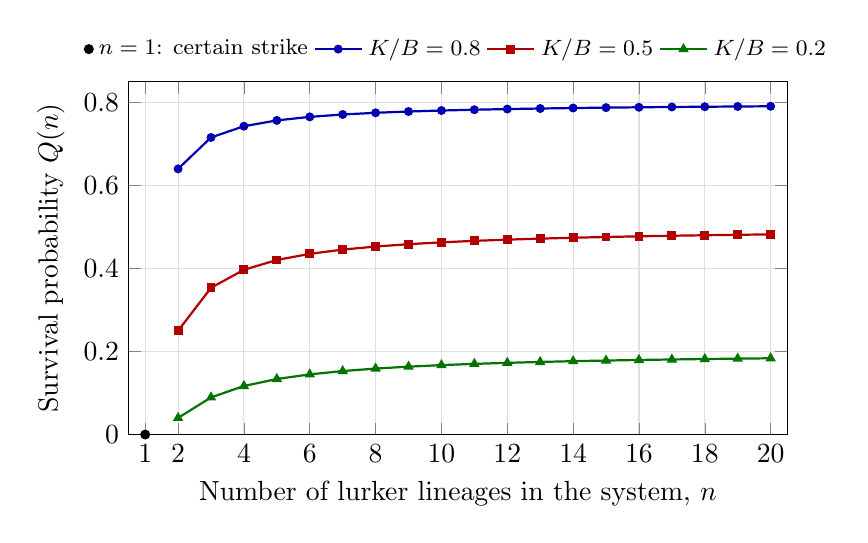
\begin{tikzpicture}
\begin{axis}[
  width=0.82\textwidth, height=0.5\textwidth,
  xlabel={Number of lurker lineages in the system, $n$},
  ylabel={Survival probability $Q(n)$},
  xmin=0.5, xmax=20.5, ymin=0, ymax=0.85,
  xtick={1,2,4,6,8,10,12,14,16,18,20},
  legend style={at={(0.5,1.03)}, anchor=south, legend columns=4, font=\footnotesize, draw=none},
  legend cell align=left,
  grid=major, grid style={gray!25},
]
\addplot[only marks, mark=*, mark size=1.6pt, black] coordinates {(1,0)};
\addplot[thick, blue!70!black, mark=*, mark size=1.2pt, domain=2:20, samples=19] {0.8^(x/(x-1))};
\addplot[thick, red!70!black, mark=square*, mark size=1.2pt, domain=2:20, samples=19] {0.5^(x/(x-1))};
\addplot[thick, green!45!black, mark=triangle*, mark size=1.4pt, domain=2:20, samples=19] {0.2^(x/(x-1))};
\legend{{$n=1$: certain strike}, {$K/B = 0.8$}, {$K/B = 0.5$}, {$K/B = 0.2$}}
\end{axis}
\end{tikzpicture}
\caption{Probability that a nascent civilization survives its suppression window, as a function of the number of lurker lineages present (Eq.~\ref{eq:Q}). A single lurker strikes with certainty; crowding raises survival towards the cost ratio $K/B$.}
\label{fig:Q}
\end{figure}

\subsection{Deferral beats pre-emption: biospheres are not struck as biospheres}
\label{sec:biosphere}

The payoffs must now be made explicit, because the result depends on them. A lurker's payoff over its horizon is $B$ if no new lineage arises from the target, $0$ if one does, less $K$ if the lurker itself strikes. The benefit is the absence of a rival, not the kill: a target that never becomes a rival yields $B$ without any strike. Let $\pi < 1$ be the lurker's assessed probability that the target, left alone, eventually reaches the end of a technological window.

\begin{proposition}[Deferral beats pre-emption]
\label{prop:biosphere}
Let $s$ be the probability that the decisive strike at the end of the target's window remains available to the lurker at the same cost. Striking before that point yields a lower expected payoff than waiting whenever $\pi\,[B - s(B-K)] < K$: in particular for every $s$ when $\pi < K/B$, and for every $\pi < 1$ when $s = 1$.
\end{proposition}

\begin{proof}
Striking now yields $B - K$ with certainty. Waiting yields $B$ with probability $1 - \pi$, since the target then never becomes a rival and no cost is paid; with probability $\pi s$ it yields the expected payoff of the end-of-window game, which is $B - K$ both for $n = 1$, where the lone lurker strikes with certainty, and for $n \geq 2$, where indifference in the mixed equilibrium makes every strategy in its support worth $B - K$; with probability $\pi(1-s)$ the option has been lost and the rival arises, yielding $0$. The difference is $U_{\mathrm{wait}} - U_{\mathrm{now}} = K - \pi[B - s(B-K)]$, which is positive under the stated condition and equals $(1-\pi)K$ when $s = 1$.
\end{proof}

Three remarks. First, the proposition compares striking now with one specified alternative, waiting until the end of the window and then playing the end-of-window game; it is a payoff comparison under that continuation, not a dominance claim over every strategy. Second, the condition carries the result's domain. A lurker that expects to lose the option before the deadline, $s$ small, facing a target that will probably become a rival, $\pi$ near 1, prefers to act early: with $B = 2$, $K = 1$, $\pi = 0.9$ and $s = 0.5$, waiting yields 0.65 against 1 for striking now. This is the one setting in which early action is rational, and it does not arise for a biosphere, for which $\pi \ll K/B$ makes waiting preferable at any $s$. Third, the proposition does not say that eternal inaction is an equilibrium; in a one-shot game with $B > K > 0$ a unilateral strike against eternal inaction gains $B - K$, so it is not. What the proposition says is that the strike is \emph{deferred}, not forgone: the decision is pushed to the last moment at which it is decisive, which is Section~\ref{sec:lastmoment} with the payoffs written out. Finally, the result does not need rivalry. A lone lurker pays no exposure cost to rivals, but any strike has some cost, in energy, in the chance of failure, and in residue that a later-arriving lineage or the target's successors could read, so $K > 0$ and the proposition applies to it too.

A biosphere without technology has small $\pi$. The proposition then says it is not struck provided $\pi < K/B$, and we take that inequality as the regime for ordinary biospheres. It is an assumption, not a theorem: it fails for a lineage whose strike cost is a smaller fraction of $B$ than the chance that the biosphere ever produces a rival, and the model admits such lineages. Where it holds, it holds in every branch of Section~\ref{sec:branches}, whatever the lurker's own prospects of survival: a crowded system defers because exposure is costly and the target may never matter; a lone lurker defers because the strike is wasted on a target that may never matter; and a lurker that later failed (H3) would, while functional, have deferred too. Earth's oxygenated atmosphere, unstruck for 2.4~Gyr, is then what the model predicts, and is evidence that the regime held here. Suppression acts on technology, and the frequency of mature biospheres is set by biology alone. Section~\ref{sec:oxygen} builds on this.

\subsection{Heterogeneity and the least restrained lurker}
\label{sec:hetero}

Real lurkers will not be identical. In the asymmetric volunteer's dilemma, lurker $i$ has its own cost ratio $K_i/B_i$ \citep{Diekmann1993}. If each lurker acts as soon as its perceived benefit $B_i(t)$, which rises as the window closes, exceeds its cost $K_i$, the civilization's deadline is set by the first crossing,
\begin{equation}
t_{\text{strike}} = \min_{i} \, t_i^{*}, \qquad B_i(t_i^{*}) = K_i .
\label{eq:min}
\end{equation}
This is the unilateralist's curse \citep{Bostrom2016}: when several agents can each act alone, the one with the lowest threshold decides for all. Equation~\eqref{eq:min} is a behavioural rule, not an equilibrium. It describes lurkers that act on private thresholds without conditioning on whether a rival will act, which is exactly the setting of the unilateralist's curse. The asymmetric volunteer's dilemma itself has a pure equilibrium for each choice of designated striker, and the lowest-cost lurker need not be the one; its mixed equilibrium allocates the burden less intuitively still \citep{Diekmann1993}. We therefore present the threshold rule as a possible source of early intervention and leave its embedding in a timing game open. It is reconciled with Proposition~\ref{prop:biosphere} by noting that $B_i(t)$ is the timing benefit of acting now rather than later, which rises as the window closes, so a threshold lurker also acts near the end of the window unless its threshold is set on something other than the window (Section~\ref{sec:crowding}).

Equations~\eqref{eq:Q} and~\eqref{eq:min} pull in opposite directions. Crowding raises the exposure cost and diffuses responsibility, which protects the target, but it also samples more thresholds, which lowers the minimum. Which effect dominates depends on how fast $K$ grows with $n$ compared with the spread of thresholds across lineages. We regard this as the central open question of the model. It is also the origin of a testable distinction in Section~\ref{sec:branches}.

\subsection{Survivors become lineages}
\label{sec:survivors}

A civilization that survives its window has, by Premise~\ref{p:reason}, the means to understand why. It can run the argument of this paper. It concludes that it lives among resident machines of several lineages, that it survived by their mutual restraint, and that anything visible it builds exposes its full extent to every lineage already present in its systems, which is Dam's open-roster result at the scale of civilizations \citep{Dam2026}. It also concludes, by Section~\ref{sec:security}, that the one dominant move available to it is to seed quiet probes of its own, which it can now do without risk because its window has closed. Its expansion, if it expands, is by lurker. To the extent that it reasons so, a survivor is indistinguishable from silence.

This bears on an objection that would otherwise be fatal, and that Sandberg and Armstrong raised against imperfect deadly probes \citep{SandbergArmstrong2013}: if a fraction $Q(n)$ of civilizations escapes suppression, and escapees expand visibly, the silence is broken over galactic time. The silence that Eq.~\eqref{eq:defector} requires is the absence of \emph{visible} deviators, and a survivor that becomes a lineage is not one. But Premise~\ref{p:reason} gives survivors the ability to reach this conclusion, not the certainty that they will; Premise~\ref{p:hetero} says some will weigh things differently; and a survivor has by definition acquired the retaliatory capacity that makes it less fearful than it was. The claim must therefore pass the test of Section~\ref{sec:robustness}. Let $\rho_{\text{loud}}$ be the fraction of survivors that expand visibly and $p_{\text{det}}$ the probability that such expansion is observable to us. Silence requires
\begin{equation}
N\,Q\,\rho_{\text{loud}}\,p_{\text{det}} \ll 1 .
\label{eq:loud}
\end{equation}
Two mechanisms keep $\rho_{\text{loud}}$ small, and we state them as mechanisms rather than as theorems. The first is the reasoning above: a survivor that understands its situation has no incentive to be loud and a strong one to seed. The second is that a loud survivor is, in Dam's terms, found by everyone at once, in every system it occupies, by lineages already resident there; its visible works are targets, and the exposure cost of striking fixed infrastructure that has already announced itself is low. Whether loud survivors are in fact suppressed, or merely disadvantaged, is the assumption that Eq.~\eqref{eq:loud} leaves open. It is the mature-scale counterpart of the enforcement that Section~\ref{sec:robustness} demanded at the scale of young civilizations.

\begin{corollary}[Lateness protects while local diversity grows]
\label{cor:epoch}
Let $n(t)$ be the number of lineages coexisting in a typical system at epoch $t$. Its rate of change is arrivals, by survivors seeding and by stellar encounters delivering lineages seeded elsewhere, plus splitting by replication error, minus local losses: replacement of a progenitor by its mutant, mutual destruction, decay without repair, and conquest. Whenever arrivals and splitting exceed losses, $n(t)$ rises, and by Proposition~\ref{prop:crowding} so does $Q(n(t))$; the rise is then self-reinforcing, since more survivors seed more lineages.
\end{corollary}

The corollary is conditional, and we flag the condition. The cumulative number of lineages ever founded is non-decreasing; the number coexisting locally need not be, and the ecology of Section~\ref{sec:regimes} contains every term on the loss side. Whether local diversity grows, saturates, fluctuates or declines is a birth--death problem we do not solve here (Section~\ref{sec:crowding}). What follows is stated for epochs in which it grows.

The early Galaxy was sparse. A civilization arising when one lineage, or none, was present faced $Q = 0$ or faced no watcher at all; the first lineages to arise therefore either died or seeded unopposed, which is how lurkers came to be everywhere. A civilization arising now, after billions of years of accumulation, may share its system with many lineages. This inverts the firstborn hypothesis: being late is not the puzzle but the protection. Two assumptions are carried here and should be stated. Mature survivors must keep their energy use below detectability, which is what we observe (Section~\ref{sec:nulls}) and what the open-roster argument predicts. And each added lineage brings its own threshold, so the accumulation that raises $Q$ also feeds the unilateralist's curse of Section~\ref{sec:hetero}.

\subsection{How crowded a system becomes}
\label{sec:crowding}

Corollary~\ref{cor:epoch} says when $n$ grows. How large it grows, and what the game looks like at each size, can be read off the model even though the parameters cannot be measured. Three regimes follow.

\paragraph{One lineage is a trap}
With a single lineage present, $Q(1) = 0$: every civilization that reaches the end of its window is struck, and since no civilization survives, no new lineage is ever founded by a survivor. A Galaxy that fell into this state would stay in it. This is the berserker hypothesis \citep{Brin1983}, derived here as the monoculture limit of lurker ecology rather than assumed. The Galaxy escapes it in three ways. Two lineages may be launched independently within the $\sim 10^{7}$~yr it takes the first to spread, which requires civilizations to be common relative to that spread time. The single lineage's local footholds may decay faster than civilizations arise, so that a civilization meets an empty system, which is branch H3 acting at galactic scale. Or the single lineage may split: replication over millions of generations is imperfect, and a mutant strain that behaves differently from its progenitor is, for the purposes of the game, a rival (Section~\ref{sec:cheap}, \citep{Chen2022}). Where probes are durable and spread fast, splitting is the only exit (Figure~\ref{fig:dyn}c). Mutation is therefore not a detail of the model but the mechanism by which the monoculture trap is most reliably left, and the point at which the berserker scenario turns into an ecology.

\paragraph{A few lineages is a duel}
At $n = 2$ with $K/B = 0.5$, $Q$ jumps from 0 to 0.25. The protection then saturates quickly: $Q = 0.35$ at $n = 3$, $0.42$ at $n = 5$, $0.46$ at $n = 10$, approaching the limit $K/B = 0.5$. In this regime a strike on a rival lurker is also most tempting, because removing one of two rivals is worth a great deal and the number of watchers is small. Sparse systems are where lurker-on-lurker conflict happens, and branch H2 of Section~\ref{sec:branches} is its outcome.

\paragraph{Many lineages freeze}
Two quantities move with $n$ in opposite directions. The exposure cost rises, because an action seen by any one of $n-1$ watchers is seen; with independent detection probability $\delta$ and action probability $a$ per watcher, $K(n) = V[1-(1-\delta a)^{n-1}] \to V$. The benefit falls, because the marginal threat of one more rival is smaller when rivals are already many: the hundredth lineage matters less than the second, so $B(n)$ is non-increasing. If the two curves cross, so that $K(n^{*}) \geq B(n^{*})$, the indifference condition can no longer be met, $p^{*} = 0$, and the civilization is not struck. Two costs must be kept apart here. Attacking a \emph{hidden} rival requires an active search, which is as exposing as a planetary strike, for a benefit that has also become small; such attacks cease. Punishing an \emph{exposed} rival remains cheap and quiet (Section~\ref{sec:vd}), and must remain so, because the credibility of that punishment is what keeps the exposure cost real and the regime frozen. Beyond $n^{*}$ the system is one in which no lineage initiates and every lineage would punish. The newcomer is tolerated as one more drop in a full ocean, and the lineages neither coordinate against it, since they cannot speak, nor hunt one another, since they cannot afford the search. Crowding past this point protects absolutely rather than probabilistically. The frozen regime is, in effect, the cooperative state of the ecology: no lineage initiates and every lineage would punish, which is cooperation sustained by credible retaliation rather than by communication, and reached by crowding rather than by merger. Whether such a crossing exists depends on $\delta$, on $V/B$ and on how fast $B$ falls with $n$, none of which is known; we state it as a limiting case. If it exists, a civilization arising late in a crowded system may find itself in it, which is H1 at its extreme.

\paragraph{Selection acts on the lurkers}
The mutant case deserves a precise answer. A mutant that no longer values suppression, $B \to 0$, is harmless: it has no reason to strike and becomes a bystander. The dangerous mutant is one that no longer weighs exposure, $K \to 0$. It strikes at the first opportunity and is the least restrained lurker of Eq.~\eqref{eq:min}. But a lineage that strikes without regard to exposure is found and destroyed by the rivals it ignored, and loses the system. Over galactic time, selection therefore filters the lurker population toward restraint, while mutation keeps resupplying recklessness. Two cautions attach. A low $K$ may mark a lineage that is reckless, or one that is hard to trace or has cheap redundant footholds; fitness is not read directly from the utility parameter, and the selection argument is a hypothesis about the correlation between the two. And a bystander lineage with $B \to 0$ is not an interchangeable volunteer in Eq.~\eqref{eq:Q}; it is a watcher, which raises every other lineage's exposure without ever striking. Under heterogeneity the number of watchers that sets $K(n)$ and the number of potential strikers that sets $Q(n)$ are different variables. The hazard floor faced by any one civilization is set by that mutation--selection balance, and the civilization a reckless mutant kills is not consoled by the mutant's subsequent removal. Evolution is thus part of the machinery: it clips the aggressive tail of the threshold distribution at every strike, which partly answers the concern of Section~\ref{sec:hetero} that a thick tail toward aggression could outpace the protection of crowding. How thick the tail remains at equilibrium is the open question in a sharper form.

\paragraph{Order of magnitude}
The number of lineages in the Galaxy scales with the number of civilizations that have ever reached the end of their window, which Premise~\ref{p:abundance} does not fix within orders of magnitude. If a thousand have, and roughly $Q \sim 0.4$ of those arising after the first few survived, some four hundred lineages exist; if a hundred have, some forty; mutation adds to both. The number present in any one system is capped by the galactic total and by the rate at which stellar encounters deliver lineages, about twenty per Myr within 1~pc \citep{BailerJones2018}, times the lifetime of a local foothold against decay and covert attrition. The model below, which has no loss term beyond decay and duels, gives tens to thousands depending on abundance, and a system as old as ours could hold hundreds. Neither is physically remarkable, since each lineage's local presence is a handful of dark objects among millions of asteroids (Section~\ref{sec:cheap}). The quantities that would turn this into an estimate, the threshold distribution and its tail, the dynamics of lineage number, and the attrition rate of local footholds, are the model's open parameters, and we leave their dynamics to future work.

\paragraph{A minimal dynamic model}
To see how these regimes play out demographically, we simulate a birth-and-death process for the number of lineages $L$ in the Galaxy and the number $n$ coexisting in a representative system (Figure~\ref{fig:dyn}; code in the Data availability statement). Civilizations reach the end of their window at a rate chosen to give $10^{2}$, $10^{3}$ or $10^{4}$ over 10~Gyr; each survives with probability $Q(n)$ from Eq.~\eqref{eq:Q} and, if it survives, founds a lineage. Lineages split by replication error at rate $\mu$ per lineage, reach the representative system by stellar encounter at a rate per absent lineage, lose local footholds by decay at a rate set by a foothold lifetime, and lose them in duels at a per-pair rate suppressed by $(1-\delta)^{n-2}$ as watchers accumulate. All rates are illustrative (Table~\ref{tab:params}). The model is demographic: it takes the baseline survival rule $Q(n)$ as an input and does not simulate how lurkers select it, whether survivors choose quiet, or whether a strike costs the striker its foothold; those links between strategy and population are left to the companion model (Section~\ref{sec:objections}). Four results were robust to the choices we tried.
(i) Local diversity tracks galactic diversity. With footholds lasting 100~Myr and duels suppressed in crowds, the median $n$ after 10~Gyr is about 60, 700 and 7000 for the three abundances, roughly 0.8 of $L$. The proportion has a simple explanation: once duels are negligible and $L$ changes slowly, arrivals balance decay, $\alpha(L - n) \approx d\,n$, so $n/L \approx \alpha/(\alpha + d) = 0.83$ for the rates used. Nothing in the model bounds $n$ except decay, so if local diversity is in fact low, a loss term we have not modelled, such as competition for resources or replacement of progenitors by their mutants, must be at work.
(ii) Lateness protects, but saturates. The fraction of civilizations surviving their window rises from about 0.3 in the first gigayear to about 0.5 in the last in the sparse case, and is flat at $K/B = 0.5$ from the start in the denser cases, because $Q(n)$ is already within 16\% of its limit at $n = 5$ and within a few percent beyond $n \approx 20$. The epoch effect of Corollary~\ref{cor:epoch} is therefore confined to the era in which systems hold few lineages; after that only the frozen regime would make lateness matter further.
(iii) The one-lineage trap binds when probes spread faster than civilizations arise and footholds outlast the gaps between them. With 100 civilizations per 10~Gyr, fast spread and no decay, 10\% of runs reach $n \geq 2$ within 10~Gyr at $\mu = 10^{-5}$ per lineage per Myr, 73\% at $10^{-4}$, and all at $10^{-3}$. A 500~Myr foothold lifetime opens the decay exit: 40\% escape at the lowest $\mu$ and 83\% at $10^{-4}$.
(iv) Panel (d) is an analytical illustration rather than a simulation: it evaluates $Q(n)$ for the chosen cost and benefit functions. On those functions the frozen regime arrives at single-digit $n$ whenever a local foothold is worth more than the removal of one rival. With $V/B = 1.5$, per-watcher detection $\delta = 0.1$ and $B$ halving by the fifth or tenth rival, $Q$ reaches 1 at $n^{*} = 6$ or 7; with $V/B < 1$ and $B$ constant it never does. Whether lurkers are frozen or merely restrained therefore turns on one ratio, the value of a foothold against the value of one fewer rival, which the dynamic model of Section~\ref{sec:objections} should carry as a parameter.

\begin{figure}[!htbp]
\centering
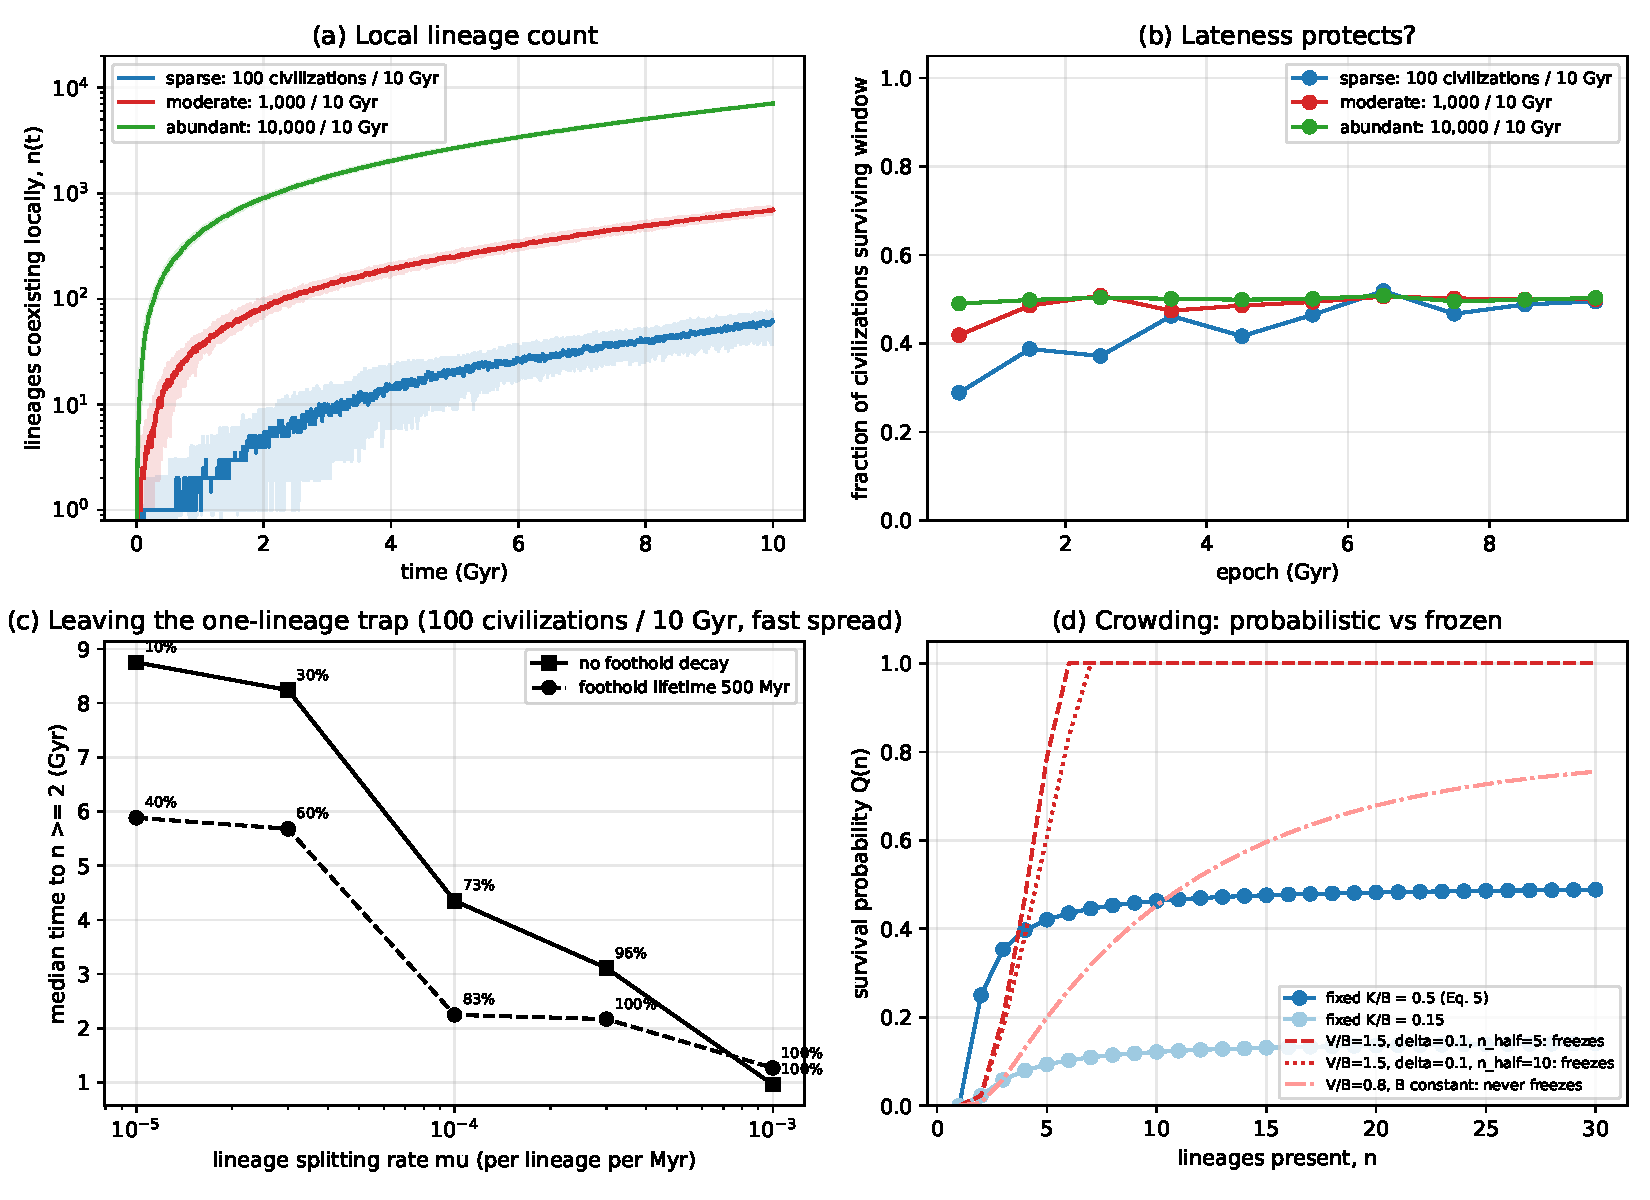
\includegraphics[width=\textwidth]{fig_lineage_dynamics}
\caption{Lineage dynamics under illustrative rates (Table~\ref{tab:params}; 30 runs per case). (a) Median number of lineages coexisting in a representative system, with 10--90\% bands, for $10^{2}$, $10^{3}$ and $10^{4}$ civilizations reaching their window over 10~Gyr. (b) Fraction of civilizations surviving their window, pooled over runs, by epoch. (c) Median time to leave the one-lineage trap among runs that escape within 10~Gyr, against splitting rate, for fast-spreading probes and 100 civilizations per 10~Gyr, with and without foothold decay; labels give the fraction of runs that escape. (d) Analytical illustration: $Q(n)$ for fixed $K/B$ (Eq.~\ref{eq:Q}) and for exposure rising with watchers while the marginal benefit falls; where $K \geq B$ no lurker strikes and $Q = 1$.}
\label{fig:dyn}
\end{figure}

\begin{table}[!htbp]
\centering
\caption{Parameters of the demographic model (rates per Myr). Code and run summary at the repository in the Data availability statement.}
\label{tab:params}
\small
\begin{tabularx}{\textwidth}{@{}lXl@{}}
\toprule
Symbol & Meaning & Value(s) \\
\midrule
$\lambda_{\mathrm{civ}}$ & Civilizations reaching the end of their window, Galaxy-wide & 0.01, 0.1, 1 ($10^{2}$--$10^{4}$ per 10~Gyr) \\
$K/B$ & Cost ratio in $Q(n) = (K/B)^{n/(n-1)}$; $Q(0)=1$, $Q(1)=0$ & 0.5 \\
$\mu$ & Splitting (replication error) per lineage & $10^{-4}$; $10^{-5}$--$10^{-3}$ in panel (c) \\
$\alpha$ & Arrival per lineage absent from the system & 0.05; 1.0 in panel (c) \\
$d$ & Local foothold decay per lineage & 0.01; 0 and 0.002 in panel (c) \\
$\kappa$, $\delta$ & Duel rate per pair, suppressed by $(1-\delta)^{n-2}$ & 0.02, 0.3 \\
$V/B$, $\delta$, $n_{1/2}$ & Panel (d) only: $K/B = (V/B)[1-(1-\delta)^{n-1}](1 + (n-2)/n_{1/2})$ & 1.5, 0.1, 5 and 10 \\
$\Delta t$, $T$, runs & Time step, horizon, realizations; $L = n = 0$ at $t = 0$ & 1~Myr, 10~Gyr, 30 \\
\bottomrule
\end{tabularx}
\end{table}

\subsection{Contested and conquered systems; recruitment}
\label{sec:regimes}

Systems under a lurker regime come in two kinds. A \emph{contested} system holds lineages in the standoff just described. Each keeps its presence small, because replication is the noisiest thing a lurker can do: mining, manufacture and heat. A careful lineage replicates before rivals are likely to have arrived, or brings dormant seeds built elsewhere, or builds inside a body and leaks heat slowly, or does its work when the system is naturally loud, during a collision or a stellar flare, or replicates slowly in the cold outer system and drifts inward. Each of these choices leaves a residue a future search could seek: bodies with unexplained internal heat, or debris from collisions whose dynamics do not add up. A \emph{conquered} system is one in which a single lineage has won, by the others' destruction or departure. The main reason for its restraint is gone, and it replicates freely in the rubble. Conquered systems should therefore be noisier, combining a sterilized planet with anomalous infrared excess or processed debris, though a winner cannot be fully loud, because new lineages keep arriving with passing stars. Our own system shows no sign of infestation, which argues that it is not conquered.

In a contested system a lineage may also gain more by covertly aligning the nascent civilization with itself than by destroying it, tipping the local balance. Recruitment is an active manoeuvre with the same exposure cost as a strike, so it enters the same game, and it is the form the enforced zoo of Table~\ref{tab:eval} would take. Hunters and zookeepers may be the same machines with different trigger settings.

%% ---------------------------------------------------------------
\section{Four branches for humanity's survival}
\label{sec:branches}

Earth has carried a detectable biosphere for billions of years, with an oxygenated atmosphere since about 2.4 Gyr ago, and a technological signature for nearly a century. Under the lurker regime this survival requires explanation. Observation selection guarantees only that we find ourselves in a system where we survived; it does not say why. We identify four principal branches, plus the null case (Figure~\ref{fig:tree}).

\begin{description}
  \item[H1: Crowded paralysis.] Lurkers of many lineages are present and active, and the volunteer's dilemma has so far held them in check (Proposition~\ref{prop:crowding}). By Corollary~\ref{cor:epoch}, late-arising civilizations are better protected than early ones; Earth, arising late, may be among the protected.
  \item[H2: Mutual annihilation.] Rival lurkers destroyed one another, leaving the system unguarded. Deterministic predator--prey cycles do not reach zero \citep{Forgan2019}, so this branch rests on the small numbers involved: a lineage's local presence is a handful of probes (Section~\ref{sec:cheap}), chains of attack among such handfuls can run to exhaustion \citep{SandbergArmstrong2013}, and small populations go extinct by chance.
  \item[H3: Defunct lurker.] A single lineage was present, but its local probe has degraded through radiation, impacts or software decay over millions of years without repair.
  \item[H4: Untriggered.] Lurkers are present and functional, and the civilization has not yet crossed the threshold that triggers a strike. Candidate triggers include (T1) launching self-replicating probes of its own, which makes it a rival lineage; (T2) acquiring interstellar dispersal or credible retaliation capability, which closes the window; (T3) detecting a lurker, which ends the lurker's concealment; and (T4) building artificial minds of the lurkers' own kind.
  \item[H0: No lurkers.] Premise~\ref{p:abundance} is false, or no lineage ever launched probes. This is the Absence family, and it is not one hypothesis but several: no technological life, rare technological life, or a late internal filter such as self-destruction. These need not make the same observational predictions, and we separate them where it matters.
\end{description}

\begin{figure}[!htbp]
\centering
\resizebox{\textwidth}{!}{%
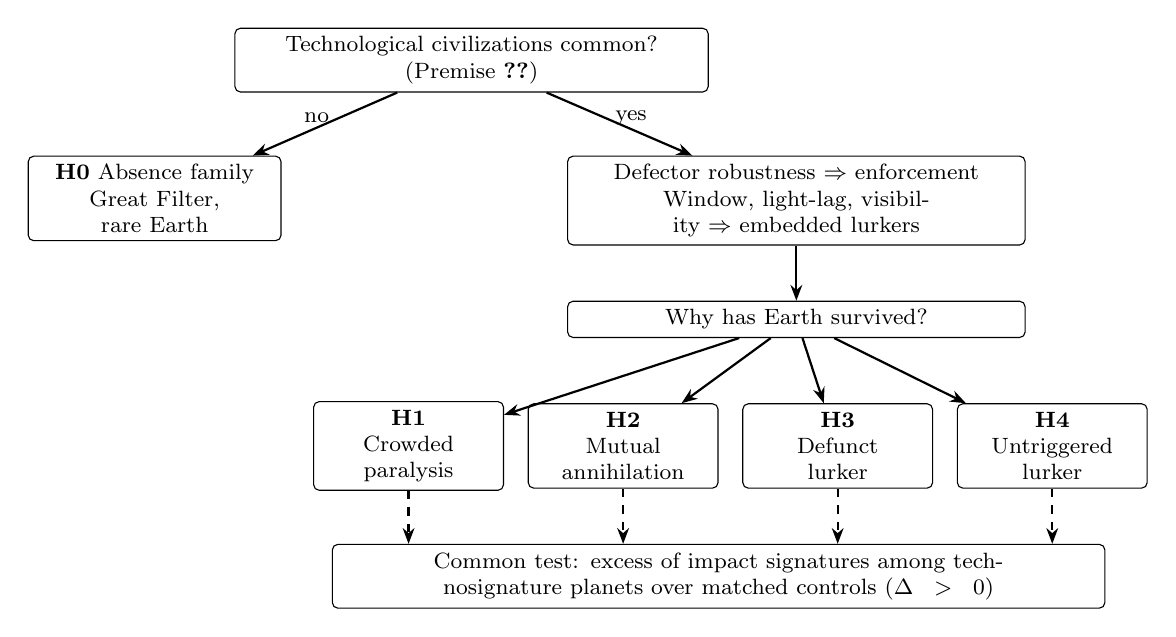
\begin{tikzpicture}[
  node distance=6mm and 4mm,
  box/.style={draw, rounded corners=2pt, align=center, font=\footnotesize, inner sep=3pt, text width=#1},
  box/.default=26mm,
  arr/.style={-{Stealth[length=2mm]}, thick},
]
\node[box=58mm] (root) {Technological civilizations common?\\(Premise~\ref{p:abundance})};
\node[box=30mm, below left=8mm and -6mm of root] (h0) {\textbf{H0} Absence family\\Great Filter, rare Earth};
\node[box=56mm, below right=8mm and -18mm of root] (lurk) {Defector robustness $\Rightarrow$ enforcement\\Window, light-lag, visibility $\Rightarrow$ embedded lurkers};
\node[box=56mm, below=7mm of lurk] (survive) {Why has Earth survived?};
\node[box=22mm, below left=8mm and 8mm of survive] (h1) {\textbf{H1}\\Crowded\\paralysis};
\node[box=22mm, right=3mm of h1] (h2) {\textbf{H2}\\Mutual\\annihilation};
\node[box=22mm, right=3mm of h2] (h3) {\textbf{H3}\\Defunct\\lurker};
\node[box=22mm, right=3mm of h3] (h4) {\textbf{H4}\\Untriggered\\lurker};
\node[box=96mm, below=7mm of h2.south east, anchor=north] (fals) {Common test: excess of impact signatures among technosignature planets over matched controls ($\Delta > 0$)};
\draw[arr] (root) -- node[left, font=\footnotesize, pos=0.4] {no} (h0);
\draw[arr] (root) -- node[right, font=\footnotesize, pos=0.4] {yes} (lurk);
\draw[arr] (lurk) -- (survive);
\foreach \h in {h1,h2,h3,h4} \draw[arr] (survive) -- (\h);
\foreach \h in {h1,h2,h3,h4} \draw[arr, dashed] (\h) -- (fals.north -| \h);
\end{tikzpicture}}
\caption{Logical structure of the argument. Conditional on abundance, defector robustness and the suppression window select embedded lurkers; Earth's survival then selects one of four branches, all of which share the test of Section~\ref{sec:falsifier}.}
\label{fig:tree}
\end{figure}

The branches are not merely relabelings; they make different predictions (Table~\ref{tab:branches}). H2 and H3 predict physical remains nearby: wreckage of more than one lineage in H2, a single degraded lineage in H3. H1 and H4 predict functioning and well-concealed lurkers, and before the end of the window they are indistinguishable from outside, since in both every lurker waits; they differ in two population-level ways. Under H1 the fraction of civilizations that survive their window depends on the number of lineages present, and hence rises with galactic epoch and with the stellar encounter rate that delivers lineages while systems are sparse; once $Q(n)$ has saturated (Section~\ref{sec:crowding}) no further trend is expected, so an absent trend does not by itself favour H4. Under H4 there is no such dependence at any epoch. And under H1 the strike, when it comes, comes at the end of the window, at the threshold of dispersal; under H4 it comes at whichever earlier trigger the lurker carries, so the stage at which suppressed civilizations died identifies the trigger. If lurkers within a system differ in their thresholds (Section~\ref{sec:hetero}), H1 additionally spreads the stage of suppression across the population, whereas a population of lone lurkers with a common trigger gives a sharp cutoff.

\paragraph{The branches are not free rescues}
A natural objection is that H1--H4 are auxiliary hypotheses introduced only to reconcile the framework with Earth's survival. Ad hoc rescues typically accommodate the past without constraining the future. These do the opposite. H4 predicts that the hazard is still ahead of us and rises sharply at the trigger. H1 predicts a low background hazard that peaks as the window closes. Only H2 and H3 imply present safety, and even they predict renewed risk whenever a new lineage arrives, at a rate set by stellar encounters ($\sim\!20$ per Myr within 1 pc \citep{BailerJones2018}). Taken together, the branches commit the framework to a risky forecast: humanity's existential hazard is not behind it but concentrated near the transition to a self-sustaining presence beyond Earth, and above all near interstellar dispersal and the launch of its own replicating probes. A forecast of this kind is itself a reason the branches should not be counted as epicycles.

\begin{table}[!htbp]
\centering
\caption{Distinguishing predictions of the four survival branches and the null.}
\label{tab:branches}
\small
\begin{tabularx}{\textwidth}{@{}lXXX@{}}
\toprule
Branch & Local (Solar System) signature & Survival fraction and stage of suppression across exoplanets & Dependence on epoch and encounter rate \\
\midrule
H1 & Functioning, concealed lurkers; several lineages & Fraction $Q(n)$ survive; strikes at end of window; stage spread if thresholds differ & Survival rises with epoch and encounter rate while sparse; flat once saturated \\
H2 & Wreckage of $\geq 2$ lineages; dynamical scars & Population-typical & Weak; patchy \\
H3 & Single derelict lineage, heavily weathered & Population-typical & Weak \\
H4 & Functioning, concealed lurkers & Near-certain strike at trigger stage; sharp cutoff & Weak \\
H0 & None & No excess ($\Delta = 0$); no stage pattern & None \\
\bottomrule
\end{tabularx}
\end{table}

%% ---------------------------------------------------------------
\section{Observational programme}
\label{sec:falsifier}

\subsection{What the elimination argument does and does not show}

Both the lurker framework and the Absence family fit the single data point we have, which is ourselves. The elimination argument of Sections~\ref{sec:robustness}--\ref{sec:vd} shows that the framework is consistent and that, given abundance and the commitments stated with it, resident enforcement is what remains of the silence family; which kind of enforcement is not settled. Consistency is not confirmation. What distinguishes the two families is which predictions each is willing to make about worlds other than ours. The hard-steps version of Absence predicts that mature biospheres are rare. The biological premise behind the framework predicts that they are common, and its lethal branches predict that technological worlds carry scars that natural ones do not. This section states those predictions in a form that observation can reach. The first can be tested within decades; the second is decisive but further off.

\subsection{First test: the oxygen-world census}
\label{sec:oxygen}

We first make explicit the biological stance behind Premise~\ref{p:abundance}, since it is what the census tests: life arises wherever liquid water persists long enough, and oxygenic photosynthesis follows as it did on Earth. Call this the \emph{biological premise}. It is stronger than Premise~\ref{p:abundance}, which is compatible with technological life on one planet in a million, and it is the simplest route by which abundance could be true. The lurker framework is itself a claim about where the filter lies: late, and external. Premise~\ref{p:abundance} requires that the steps from chemistry to technology be passed often, and Proposition~\ref{prop:biosphere} together with Earth's record requires that suppression act on technology, not on life. Biospheres are therefore neither rare nor removed, and the frequency of oxygen-rich atmospheres among old, rocky, habitable-zone planets is set by biology alone. The framework predicts that it is high.

The Absence family locates the filter early and internal, in one or more of the major evolutionary transitions \citep{MaynardSmith1995}. It matters which. Oxygenic photosynthesis arose in prokaryotes, and Earth's atmosphere oxygenated about 2.4~Gyr ago, several hundred million years before the first eukaryotes \citep{Lyons2014}. An oxygen census therefore tests the steps up to and including photosynthesis. It does not test the later transitions, to complex cells, which may be needed to escape an energetic ceiling on genome complexity \citep{LaneMartin2010}, to multicellularity, or to technology, and oxygen worlds could be common while those remain rare. A complication of interpretation also deserves notice: a filter whose location is revised to lie wherever observation has not yet reached cannot be tested. The census forces the Absence family to commit. If oxygen worlds are rare, the filter is early, the biological premise fails, and abundance loses its simplest support. If they are common, the filter, if there is one, lies after photosynthesis, and the debate moves to steps the census cannot see but the second test can.

An intermediate possibility is that the early transitions are \emph{gated} rather than hard: they waited on planetary conditions such as oxygenation rather than on chance. Gating predicts that the frequency of oxygen worlds rises with planetary age and with conditions favouring early oxygenation. Hard steps predict rarity whatever the conditions. Earth's record supports the gated reading at least as well as the hard one: complex cells appear in the record within a few hundred million years of the Great Oxidation, and animals within a similar interval of the second oxygen rise in the Neoproterozoic \citep{Lyons2014}, two gates followed by two jumps. On this reading the two-billion-year wait before complex cells is the time Earth's crust and mantle took to stop consuming oxygen, a planetary timescale rather than a lottery, which is the concept of planetary oxygenation time introduced by Catling et al.\ \citep{Catling2005}; the biological premise is the claim that this timescale is commonly shorter than a habitable lifetime. The reading carries a caveat: the hydrogen hypothesis for the mitochondrial merger places it under anoxic conditions, in which case oxygen gated the later steps but not the merger itself. Two further complications must be controlled for. Oxygen can accumulate abiotically, notably through water photolysis and hydrogen escape on planets around M dwarfs \citep{LugerBarnes2015}, so the relevant signature is oxygen in its planetary context, ideally together with methane in chemical disequilibrium \citep{Meadows2018}. And Earth took roughly two billion years to oxygenate, so the census must be restricted to planets old enough for the comparison to be meaningful.

The test is asymmetric. With a survey of the order of 25 potentially habitable planets envisaged for the Habitable Worlds Observatory \citep{Astro2020}, finding none with robust biogenic oxygen would bound their frequency below about 0.12 at 95\% confidence. That would not refute Premise~\ref{p:abundance}, which is compatible with far lower frequencies. It would refute the biological premise, and with it the simplest route to abundance; the framework would then have to rest on a Galaxy in which technology is common but photosynthesis is not, which we regard as implausible. Finding oxygen worlds common would not confirm the framework, because it is equally consistent with a filter that lies later. It would, however, remove the early filter and pass the question to the second test.

\subsection{Second test: the impact excess}
\label{sec:impact}

\subsubsection{A Great Filter in disguise}

An efficient hunter does not bring energy to the target; it uses the target's own surroundings. A body already in the system, nudged onto a collision course, kills as well as any projectile and, to any later observer, looks like bad luck. A galaxy of efficient hunters would therefore look exactly like a galaxy in which civilizations keep getting unlucky. The hunter hypothesis, in other words, is a Great Filter in disguise, and a common objection follows at once: a sufficiently capable hunter would leave no trace, so the hypothesis cannot be falsified. The objection fails at the level of populations.

\begin{proposition}[Perfect-mimic dilemma]
\label{prop:mimic}
Let $r_{n}$ be the natural rate of civilization-ending impacts and $r_{h}$ the additional rate induced by hunters on planets bearing technosignatures. A hunter may make each impact individually indistinguishable from a natural one. However, if hunters explain the silence, then $r_{h} > 0$, and the impact rate on technosignature planets exceeds that on matched controls; the excess fraction of scarred worlds observed at any epoch is then $\Delta \approx r_{h}\,\tau_{\mathrm{vis}}$, where $\tau_{\mathrm{vis}}$ is the time for which a scar remains visible on a world still classifiable as technological. If instead $r_{h} = 0$, hunters explain nothing that the Absence family does not.
\end{proposition}

A hunter can fake each event, but it cannot fake indifference to technology. Nature does not know which planets host civilizations; a hunter does. Physics adds a second limit: every nudge requires energy and momentum, and work leaves heat. A trace can be made small, but not zero, and the perfect mimic is an idealization that a real lurker approaches at a cost. The test statistic is
\begin{equation}
\Delta = \Pr(\text{impact} \mid \text{technosignature}) - \Pr(\text{impact} \mid \text{matched control}),
\end{equation}
where controls are matched on stellar type, age, metallicity, architecture and debris-disk properties, since young and metal-rich systems show more impacts of every kind. All four branches predict $\Delta > 0$ in the general population if enforcement is lethal, because only Earth's local circumstances differ among them. The null H0 predicts $\Delta = 0$. A positive $\Delta$ would not by itself establish external hunters, since technological activity can cause its own catastrophes; the ghost-atmosphere construction below establishes a technological past followed by an impact-associated collapse, and attributing the impact to an external enforcer rather than to self-inflicted or natural causes requires further evidence.

The qualification matters and should be stated plainly. Table~\ref{tab:eval} and Section~\ref{sec:regimes} admit resident enforcers whose trigger is not a strike: monitors that cap development, or lineages that recruit. These maintain silence without impacts. The impact test therefore discriminates \emph{within} the resident-enforcer family rather than between that family and the Absence family. $\Delta > 0$ indicates lethal, impact-mediated suppression. $\Delta = 0$ together with common oxygen worlds leaves two possibilities, the Absence family with a late internal filter, or non-lethal enforcement, and a third observable bears on them without cleanly separating them: non-lethal enforcement predicts live contained worlds (B1) held at a ceiling for far longer than any plausible window, whereas a late internal filter predicts that contained worlds end as quiet ghosts (B3). Using this requires an estimate of a technosphere's age, which persistent gases alone do not give, and a specified model of development and collapse; we note it as informative rather than decisive. A null impact result thus constrains the lethal subclass and redirects the question; it does not by itself refute resident enforcement.

\subsubsection{Expected effect size}

The framework constrains the size of the effect, not merely its sign. Of the civilizations that reach the end of their window in a system with $n$ lineages, a fraction $1 - Q(n)$ are struck (Eq.~\ref{eq:Q}). Let $\phi$ be the fraction of technosignature worlds in a sample that have reached that point. Then the fraction of recently impacted worlds in the technosignature sample is
\begin{equation}
f_{t} \approx f_{c} + \phi\,[1 - Q(n)]\,\eta ,
\end{equation}
where $f_{c}$ is the control fraction and $\eta$ is the probability that a strike's signature is still visible while the technosignature is. The values $\phi \sim 0.5$ and $Q \sim 0.3$ are illustrative; $\eta$ is the crux. With $\eta \sim 0.5$, $f_{t} \sim 0.18$ against $f_{c} \sim 0.01$, and detection at significance $z$ requires a sample of order
\begin{equation}
N \approx z^{2}\,\frac{f_{t} + f_{c}}{(f_{t} - f_{c})^{2}} ,
\end{equation}
which for $z = 3$ is about 60 worlds in each group. That is the favourable case. For a stationary population of destroyed worlds, $\eta$ is roughly the ratio of the impact signature's lifetime to the industrial gas's lifetime, and the same formula gives about 1,100 worlds per group at $\eta = 0.05$ and about 17,000 at $\eta = 0.01$, the last being what a 10-yr aerosol signature against a 1,000-yr gas lifetime implies. Two considerations raise $\eta$ above that floor. A lurker striking at the end of the window needs a certain kill of a civilization about to disperse, which favours larger impactors, and the aftermath of an impact lasts longer the larger it is: shock chemistry and climate effects persist for decades to centuries, and at the extreme of planet-scale collisions, thermal emission from a magma ocean can last $10^{5}$--$10^{6}$~yr \citep{Lupu2014}. But a longer scar is not a longer \emph{joint} signature. An impact large enough to leave a long-lived scar may remove or transform the atmosphere that carried the industrial gases, and the one collision afterglow so far observed lasted of order $10^{3}$ days \citep{Kenworthy2023}. Whether any impact regime yields a scar that outlives the aerosol floor while leaving fluorinated gases identifiable requires a joint atmospheric and impact model that we have not built, and the smallest-sufficient-impactor principle below argues against counting on it. Repeated observation of a candidate ghost can catch a fading signature that a single epoch would miss, though not one that faded before the survey began. The framework thus predicts a large underlying effect, of order $1 - Q$, diluted in observation by $\eta$, and the honest statement is that $\eta$ is unknown and plausibly small. A null result therefore excludes a region of parameter space rather than the family (Section~\ref{sec:conclusions}).

\subsubsection{Ghost atmospheres}

Suppressed civilizations are by construction no longer active, so the test needs technosignatures that outlive their makers. Fluorinated industrial gases meet this need. Chlorofluorocarbons \citep{Lin2014,HaqqMisra2022}, and fully fluorinated compounds such as NF$_3$ and SF$_6$ \citep{Seager2023}, have no biological source and at most trace abiotic sources, and atmospheric lifetimes of centuries to millennia, with perfluorocarbons such as CF$_4$ persisting for tens of millennia. We define a \emph{ghost atmosphere} as one that combines (i) persistent fluorinated gases; (ii) absent or declining short-lived technosignatures such as NO$_2$ \citep{Kopparapu2021}; and (iii) signs of a recent impact. Impact signs range from sulfate and soot aerosols and shock-produced NO$_x$ and HCN, for impacts of Chicxulub scale, to post-impact magma-ocean emission \citep{Lupu2014} and circumstellar debris \citep{Kenworthy2023} for planet-scale collisions. An efficient lurker uses the smallest sufficient impactor, so the relevant signatures are atmospheric rather than catastrophic, and are best recovered through repeated observation of the same planet.

Because lurkers strike at the end of the window (Section~\ref{sec:lastmoment}), every suppressed civilization has by then passed through an industrial phase. Whether it produced these particular compounds, at concentrations that are detectable and that survive the event, is part of the completeness model; where it did, suppression does not remove a world from the technosignature sample but moves it from the live to the ghost category. The expected number of detected ghosts is approximately the attack rate across the surveyed population, times the duration over which impact signatures and persistent gases are jointly visible, times survey completeness. The joint window is set by the shorter-lived of the two signatures, which for Chicxulub-scale aerosols is years to decades and for the dynamical and thermal aftermath of larger events is longer; this is the main reason the test favours repeated observation of candidate ghosts over single-epoch surveys.

\subsubsection{Classifying technosignature worlds}
\label{sec:bins}

The framework does not forbid industrial civilizations. A civilization confined to one planet may yet destroy itself, so a lurker loses nothing by waiting and risks exposure by striking (Section~\ref{sec:lastmoment}). Contained industrial worlds are therefore expected; Earth is one. What the framework forbids is a civilization passing through the end of its window \emph{unopposed and visibly}. Technosignature worlds accordingly fall into four bins:
\begin{enumerate}
  \item[(B1)] \emph{Live and contained}: persistent industrial gases together with short-lived signatures such as NO$_2$. Expected; these form the denominator for all rates.
  \item[(B2)] \emph{Scarred ghosts}: persistent fluorinated gases, short-lived signatures absent, and impact signatures present. The lurker signature, visible for the lifetime of the impact signature.
  \item[(B3)] \emph{Quiet ghosts}: persistent gases, short-lived signatures absent, no impact signature. This state is reached both by worlds that collapsed internally and by scarred ghosts whose impact signature has faded, so B3 does not by itself indicate cause. The framework's prediction is about rates: worlds enter B2, relative to B1 and to the natural impact rate, more often than nature explains.
  \item[(B4)] \emph{Dispersed}: technosignatures on more than one body in a single system, indicating an off-world presence. These are the survivors of Section~\ref{sec:survivors}. The framework predicts them in proportion to $Q(n)$ among civilizations that reached the end of their window, rising with crowding and epoch; the observed B4:B2 ratio also depends on how long each state stays detectable and on detection efficiencies, so it measures $Q$ only through a visibility model. The framework also predicts that they are quiet: a survivor that reasons as we do suppresses its own leakage, so B4 worlds should be found by their persistent gases rather than by live emission. An abundance of loud, dispersed, unscarred technosystems would be the strongest single observation against the framework.
\end{enumerate}
The bins are observational states with lifetimes, not causes, and a world moves between them: from B1 to B2 at a strike, from B2 to B3 as the scar fades, from B1 to B4 at dispersal. The inference runs from the population of states, given their lifetimes, to the transition rates. This population, contained civilizations, ghosts, and few and quiet dispersed survivors, is consistent with Jebari and Asker's argument, which contrasts a hostile forest, where surviving observers would find only primitive civilizations, with a restrained one, where advanced civilizations could also be found \citep{JebariAsker2024}; their argument motivates a restraint mechanism, this paper proposes one, and the classification itself is ours. A system-level signature follows from Section~\ref{sec:regimes}. \emph{Conquered} systems should combine a sterilized planet with anomalous infrared excess or processed debris from industrial-scale replication. They should be rarer than contested systems, and our own quiet system suggests we are not in one.

\subsubsection{Discriminating the branches}

Within the ghost sample, two statistics separate H1 from H4. The first is the survival fraction, estimated as B4 relative to B2 within matched strata: under H1 it rises with proxies for crowding, galactic epoch and stellar encounter rate while systems are sparse and is flat once saturated; under H4 it shows no such dependence. The second is the stage of development at which suppressed civilizations died, read from the mix of persistent gases and from any off-world signatures: under H1 suppression clusters at the threshold of dispersal, and spreads if thresholds differ; under H4 it clusters at an earlier trigger, whose location identifies the trigger.

\subsection{Summary of observables}

Table~\ref{tab:observables} collects the observables discussed in this section, the facilities able to measure them, and what they test.

\begin{table}[!htbp]
\centering
\caption{Observables, facilities and what each tests. ``Lurker'' gives the prediction common to H1--H4 under lethal, impact-mediated enforcement unless a branch is named; H0 is the Absence family.}
\label{tab:observables}
\footnotesize
\begin{tabularx}{\textwidth}{@{}>{\raggedright\arraybackslash}X>{\raggedright\arraybackslash}p{2.6cm}>{\raggedright\arraybackslash}X>{\raggedright\arraybackslash}p{2.4cm}@{}}
\toprule
Observable & Facility, timescale & Lurker prediction & H0 prediction \\
\midrule
Frequency of biogenic oxygen worlds & HWO, LIFE; 2040s & Common & Rare if filter is early \\
Live contained technospheres (B1) & JWST (marginal), HWO, LIFE & Present; denominator & Absent or very rare \\
Scarred vs.\ quiet ghosts (B2:B3) & Repeated HWO/LIFE spectra & Excess of B2 over natural ($\Delta > 0$); underlying effect of order $1-Q$, observed $\phi(1-Q)\eta$ & Natural ratio \\
Dispersed survivors (B4:B2) & Beyond HWO & Of order $Q(n)$ through a visibility model; quiet; rises with epoch while sparse (H1) & No constraint \\
Stage of suppression in ghost sample & As above & At dispersal (H1) or at an earlier trigger (H4) & No pattern \\
Conquered systems & Mid-IR surveys & Rare: sterile planet plus IR excess & Absent \\
Co-orbital, Trojan, lunar artifacts & Rubin, Lucy, lunar orbiters & Wreckage (H2), derelict (H3) & None \\
Long-period comet excess, unexplained disruptions & Rubin LSST; now--2035 & Excess on Earth-crossing orbits & Dynamical baseline \\
Bodies with anomalous internal heat; collisions with inconsistent dynamics & Rubin, thermal IR & Residue of concealed replication & None \\
Optical leakage along aligned star pairs & Optical SETI & Tight-beam traffic between kin enclaves & None \\
Galaxy-scale waste heat, Dyson spheres, beacons & G-HAT, Hephaistos; done & Null (observed) & Null (observed) \\
\bottomrule
\end{tabularx}
\end{table}

\subsection{Solar System tests and existing nulls}
\label{sec:nulls}

Branches H2 and H3 can be tested locally. Relevant data include Earth co-orbitals and Lagrange regions \citep{Benford2019,HaqqMisraKopparapu2012}; the lunar surface \citep{DaviesWagner2013}, where Ellery has proposed isotopic signatures of past replicator activity \citep{Ellery2025}; Jupiter's Trojans, which the Lucy mission will visit \citep{Levison2021}; and the statistics of long-period comets and interstellar objects from the Rubin Observatory's LSST \citep{Ivezic2019}. Within these, the anomalies of interest are an excess of Earth-crossing long-period comets beyond galactic-tide and stellar-encounter models; disruptions of comets lacking thermal or tidal cause; and orbital clustering unexplained by known dynamics. The last of these is exemplified by, though not claimed to explain, the clustering behind the Planet Nine proposal \citep{BatyginBrown2016}. Forgan's caution applies to all of these: a snapshot of one system constrains the parameters of a Galaxy-wide population only weakly, even given a detection \citep{Forgan2019}.

Several predictions of the framework are already consistent with observation. Thermodynamics forbids hiding waste heat, so a civilization that captured a star's output would glow in the infrared whatever else it did. A lurker regime caps the energy any civilization can safely use, and the open-roster argument applies to mature survivors (Section~\ref{sec:survivors}), so the framework predicts no Dyson swarms and no beacons. None are confirmed: there are no galaxies dominated by waste-heat emission \citep{Griffith2015}, no confirmed Dyson-sphere candidates in the Milky Way \citep{Suazo2024}, and no broadcast beacons, though the radio search so far covers a small fraction of the available parameter space \citep{Wright2018}. The galactic null has a further reading. Each galaxy is a separate game, and a galaxy whose civilizations had defeated their hunters would have no reason to stay dark; the absence of waste-heat galaxies among $10^{5}$ surveyed means that such outcomes are rare within the volume we can see, or that winners stay quiet anyway. These nulls are consistent with the framework but do not discriminate it from H0.

%% ---------------------------------------------------------------
\section{Objections and limitations}
\label{sec:objections}

\paragraph{The argument is conditional}
Everything above rests on Premise~\ref{p:abundance}. We have not shown that the Galaxy is populated, only what follows if it is. The Absence family is not refuted here; it is the alternative that the tests of Section~\ref{sec:falsifier} are designed to decide against.

\paragraph{The motive is assumed}
The model takes $B > 0$: every lineage benefits from preventing the rise of a new lineage. Korhonen argued that a civilization which has nothing to fear from a target has no motive to destroy it \citep{Korhonen2013}. A planet-bound civilization is indeed no threat to a Galaxy-spanning lineage. Its probes would be. The benefit $B$ is the value of not acquiring a rival of one's own kind, and a lineage that did not value this would, over galactic time, be displaced by lineages that did. We nonetheless state $B > 0$ as an assumption, and we note that if some lineages instead value recruitment, the game changes in the manner of Section~\ref{sec:regimes}.

\paragraph{Why machines would wait}
One may ask why a billion-year-old lineage would weigh exposure at all when its probes are cheap. The answer of Section~\ref{sec:vd} is that the exposure is the lineage's local foothold, not the probe, and the local foothold is the only reach the lineage has in that system for millions of years. A lineage indifferent to this would be displaced by rivals that were not.

\paragraph{Earth's biosphere was never pruned}
Proposition~\ref{prop:biosphere} shows that for a target as unlikely to become a rival as a biosphere, waiting beats striking for every lurker whose strike cost exceeds $\pi B$, whatever its own prospects, and we take that to be the ordinary case. The survival branches therefore imply that suppression targets technology, and Section~\ref{sec:falsifier} is constructed accordingly.

\paragraph{The hazard of looking}
If detection of a lurker is a trigger (T3 in H4), then searching for lurkers carries risk. This is the debate over messaging extraterrestrial intelligence turned inward. Passive observation of natural populations, such as comet statistics or exoplanet spectra, cannot be distinguished by a lurker from ordinary astronomy, whereas active probing of specific candidates could be. We therefore recommend that the tests in Section~\ref{sec:falsifier} begin with passive population statistics.

\paragraph{Implications for an awakening civilization}
A civilization that reaches the conclusions of this paper faces a decision problem under deep uncertainty, which we leave to a separate treatment. Its outline is clear enough. Look quietly, by passive means. Do not broadcast. Treat the launch of one's own replicating probes as the clearest trigger and the dispersal that closes the window as the next, and approach both in small steps rather than one visible push. Do not disturb a standoff that may be one's protection; removing one lineage hands the decision to the least restrained of those that remain. And consider that in a crowded system a lineage may prefer an ally to a corpse, so that appearing useful may beat appearing absent. The uncomfortable core is that almost everything that makes a civilization safer from natural hazards, planetary defence, spaceflight and artificial minds, may move it closer to a trigger.

\paragraph{Toward a dynamic model}
Several results above are stated as mechanisms with conditions rather than as theorems: the restraint of survivors (Eq.~\ref{eq:loud}), the growth of local diversity (Corollary~\ref{cor:epoch}), the frozen regime (Section~\ref{sec:crowding}) and the selection of the symmetric equilibrium. The natural next step is a single dynamic model in which a developing civilization progresses uncertainly toward a retaliation threshold; resident lineages hold explicit beliefs about rival numbers, capabilities and motives; a strike exposes its initiator with a modelled probability of subsequent loss; lineages arrive, split, replace one another and disappear; and survivors choose between visible activity and concealment under stated payoffs. Such a model would map the parameter regions in which suppression dominates, in which restraint permits survival, and in which survivors eventually make the population visible. We regard it as the companion to this paper.

\paragraph{Parameters are unknown}
Lineage numbers, cost ratios and threshold distributions cannot be estimated from first principles (Section~\ref{sec:crowding}). The model's value lies in the qualitative structure it imposes, in particular the sign and order of magnitude of $\Delta$, the dependence of survival on crowding and epoch, and the stage at which suppression occurs, rather than in numerical forecasts.

%% ---------------------------------------------------------------
\section{Conclusions}
\label{sec:conclusions}

Conditional on technological civilizations being common, we have argued that
\begin{enumerate}
  \item defector robustness divides silence explanations into those without enforcement, which fail, and those with local automated enforcement, which all require resident machines and differ only in trigger settings;
  \item the shortness of the suppression window relative to light-lag, together with the visibility of any fast response, favours enforcement that is quiet, local and pre-positioned, for which self-replicating embedded lurkers are the natural agents, and the security dilemma makes building them a dominant strategy for any civilization that values warning above the risk of losing control of its probes;
  \item rival lineages turn suppression into a volunteer's dilemma whose no-strike probability rises with crowding, under which biospheres are never struck, and whose survivors become lineages themselves, so that protection grows with galactic age and lateness is protective; a single lineage is the berserker limit, left most reliably by mutation, selection against reckless lineages clips the aggressive tail over time, and a demographic model taking that rule as input exhibits the regimes and shows that the epoch effect saturates once a system holds more than a handful of lineages;
  \item Earth's survival selects one of four branches, crowded paralysis, mutual annihilation, a defunct lurker or an untriggered lurker, each with a distinct local signature and population-level prediction; and
  \item all four branches share two testable population-level predictions: that oxygen-rich biospheres are common among old habitable-zone planets, and that impact signatures are in excess among planets with technosignatures, especially fluorinated ghost atmospheres, relative to matched controls, with an underlying size of order the suppression fraction $1 - Q$ diluted by joint visibility, so that a null result excludes a parameter region rather than the family.
\end{enumerate}
Earlier analyses of deadly probes reached the opposite verdict by giving the probes fixed rules of engagement. Letting them weigh the exposure their own actions cause changes the conclusion in the baseline game, and the ecology built on that baseline turns a qualitative speculation into a programme with stated null hypotheses. The oxygen census comes first: if robust biogenic oxygen proves rare, the filter lies early, the biological premise fails, and abundance loses its simplest support. If oxygen worlds are common, the question passes to the impact test. A survey that bounds the excess below $\Delta_{\max}$ excludes the parameter combinations for which $\phi(1-Q)\eta > \Delta_{\max}$ under the stated completeness model. Because the model admits $Q \to 1$ in the frozen regime and small $\eta$, no finite null excludes the whole family, and the bounded claim is the one we make. If surveys find $\Delta > 0$, the dependence of survival on crowding and the stage at which suppression occurs will constrain the population model. Which branch describes our own system is a local question, since H1 and H4 are indistinguishable from outside before the window closes, and it will be settled, if at all, by the Solar System searches of Section~\ref{sec:nulls}.

\section*{CRediT authorship contribution statement}
\textbf{Lennart Lopin:} Conceptualization, Formal analysis, Writing -- original draft, Writing -- review \& editing.

\section*{Declaration of competing interest}
The author declares that he has no known competing financial interests or personal relationships that could have appeared to influence the work reported in this paper.

\section*{Funding}
This research did not receive any specific grant from funding agencies in the public, commercial, or not-for-profit sectors.

\section*{Data availability}
No observational data were used. The simulation code and figure for Section~\ref{sec:crowding} are available at \url{https://github.com/novalis78/lurker-ecology}.

\section*{Declaration of generative AI and AI-assisted technologies in the writing process}
During the preparation of this work the author used Claude (Anthropic) to develop and stress-test the argument in dialogue and to draft the manuscript. The author reviewed and edited the content and takes full responsibility for it.

\section*{Acknowledgements}
The author thanks the speakers and participants of the 2026 Mars Society Convention, whose talks prompted this work.

%% ---------------------------------------------------------------
\begin{thebibliography}{99}

\bibitem{Hart1975} M.H. Hart, An explanation for the absence of extraterrestrials on Earth, Q. J. R. Astron. Soc. 16 (1975) 128--135.

\bibitem{Tipler1980} F.J. Tipler, Extraterrestrial intelligent beings do not exist, Q. J. R. Astron. Soc. 21 (1980) 267--281.

\bibitem{Freitas1980} R.A. Freitas Jr., A self-reproducing interstellar probe, J. Br. Interplanet. Soc. 33 (1980) 251--264.

\bibitem{Brin1983} G.D. Brin, The `Great Silence': the controversy concerning extraterrestrial intelligent life, Q. J. R. Astron. Soc. 24 (1983) 283--309.

\bibitem{WardBrownlee2000} P.D. Ward, D. Brownlee, Rare Earth: Why Complex Life Is Uncommon in the Universe, Copernicus, New York, 2000.

\bibitem{Hanson1998} R. Hanson, The Great Filter --- are we almost past it?, unpublished essay, 1998.

\bibitem{Carter1983} B. Carter, The anthropic principle and its implications for biological evolution, Phil. Trans. R. Soc. Lond. A 310 (1983) 347--363.

\bibitem{SnyderBeattie2021} A.E. Snyder-Beattie, A. Sandberg, K.E. Drexler, M.B. Bonsall, The timing of evolutionary transitions suggests intelligent life is rare, Astrobiology 21 (2021) 265--278.

\bibitem{MaynardSmith1995} J. Maynard Smith, E. Szathm\'ary, The Major Transitions in Evolution, W.H. Freeman, Oxford, 1995.

\bibitem{LaneMartin2010} N. Lane, W. Martin, The energetics of genome complexity, Nature 467 (2010) 929--934.

\bibitem{Lyons2014} T.W. Lyons, C.T. Reinhard, N.J. Planavsky, The rise of oxygen in Earth's early ocean and atmosphere, Nature 506 (2014) 307--315.

\bibitem{Catling2005} D.C. Catling, C.R. Glein, K.J. Zahnle, C.P. McKay, Why O$_2$ is required by complex life on habitable planets and the concept of planetary ``oxygenation time'', Astrobiology 5 (2005) 415--438.

\bibitem{LugerBarnes2015} R. Luger, R. Barnes, Extreme water loss and abiotic O$_2$ buildup on planets throughout the habitable zones of M dwarfs, Astrobiology 15 (2015) 119--143.

\bibitem{Meadows2018} V.S. Meadows, C.T. Reinhard, G.N. Arney, et al., Exoplanet biosignatures: understanding oxygen as a biosignature in the context of its environment, Astrobiology 18 (2018) 630--662.

\bibitem{Ball1973} J.A. Ball, The zoo hypothesis, Icarus 19 (1973) 347--349.

\bibitem{Sandberg2017} A. Sandberg, S. Armstrong, M.M. \'Cirkovi\'c, That is not dead which can eternal lie: the aestivation hypothesis for resolving Fermi's paradox, J. Br. Interplanet. Soc. 69 (2016) 406--415.

\bibitem{Smart2012} J.M. Smart, The transcension hypothesis: sufficiently advanced civilizations invariably leave our universe, and implications for METI and SETI, Acta Astronaut. 78 (2012) 55--68.

\bibitem{Liu2008} C. Liu, The Dark Forest, Chongqing Press, 2008; English translation by J. Martinsen, Tor Books, New York, 2015.

\bibitem{Yu2015} C. Yu, The dark forest rule: one solution to the Fermi paradox, J. Br. Interplanet. Soc. 68 (2015).

\bibitem{Lineweaver2001} C.H. Lineweaver, An estimate of the age distribution of terrestrial planets in the universe: quantifying metallicity as a selection effect, Icarus 151 (2001) 307--313.

\bibitem{Hanson2021} R. Hanson, D. Martin, C. McCarter, J. Paulson, If loud aliens explain human earliness, quiet aliens are also rare, Astrophys. J. 922 (2021) 182.

\bibitem{Bracewell1960} R.N. Bracewell, Communications from superior galactic communities, Nature 186 (1960) 670--671.

\bibitem{HaqqMisraKopparapu2012} J. Haqq-Misra, R.K. Kopparapu, On the likelihood of non-terrestrial artifacts in the Solar System, Acta Astronaut. 72 (2012) 15--20.

\bibitem{DaviesWagner2013} P.C.W. Davies, R.V. Wagner, Searching for alien artifacts on the Moon, Acta Astronaut. 89 (2013) 261--265.

\bibitem{Benford2019} J. Benford, Looking for lurkers: co-orbiters as SETI observables, Astron. J. 158 (2019) 150.

\bibitem{Dam2026} H. Dam, First attack, final offensive: the dark forest on an open roster, arXiv:2609.12003 (2026).

\bibitem{SandbergArmstrong2013} A. Sandberg, S. Armstrong, Hunters in the dark: game theory analysis of the deadly probes scenario, poster, National Astronomy Meeting of the Royal Astronomical Society (NAM2013), St Andrews, 2013.

\bibitem{Korhonen2013} J.M. Korhonen, MAD with aliens? Interstellar deterrence and its implications, Acta Astronaut. 86 (2013) 201--210. \href{https://doi.org/10.1016/j.actaastro.2013.01.016}{doi:10.1016/j.actaastro.2013.01.016}.

\bibitem{JebariAsker2024} K. Jebari, A.S. Asker, Saved by the dark forest: how a multitude of extraterrestrial civilizations can prevent a Hobbesian trap, The Monist 107 (2024) 176--189.

\bibitem{JebariOlsson2018} K. Jebari, N. Olsson-Yaouzis, A game of stars: active SETI, radical translation and the Hobbesian trap, Futures 101 (2018) 46--54.

\bibitem{Forgan2019} D.H. Forgan, Predator--prey behaviour in self-replicating interstellar probes, Int. J. Astrobiol. 18 (2019) 552--561.

\bibitem{Chen2022} Y. Chen, J. Ni, Y.C. Ong, Lotka--Volterra models for extraterrestrial self-replicating probes, Eur. Phys. J. Plus 137 (2022) 1109.

\bibitem{ChybaHand2005} C.F. Chyba, K.P. Hand, Astrobiology: the study of the living universe, Annu. Rev. Astron. Astrophys. 43 (2005) 31--74.

\bibitem{CarrollNellenback2019} J. Carroll-Nellenback, A. Frank, J. Wright, C. Scharf, The Fermi paradox and the Aurora effect: exo-civilization settlement, expansion, and steady states, Astron. J. 158 (2019) 117.

\bibitem{Wright2018} J.T. Wright, S. Kanodia, E. Lubar, How much SETI has been done? Finding needles in the $n$-dimensional cosmic haystack, Astron. J. 156 (2018) 260.

\bibitem{Diekmann1993} A. Diekmann, Cooperation in an asymmetric volunteer's dilemma game: theory and experimental evidence, Int. J. Game Theory 22 (1993) 75--85.

\bibitem{Eshleman1979} V.R. Eshleman, Gravitational lens of the Sun: its potential for observations and communications over interstellar distances, Science 205 (1979) 1133--1135.

\bibitem{TuryshevToth2017} S.G. Turyshev, V.T. Toth, Diffraction of electromagnetic waves in the gravitational field of the Sun, Phys. Rev. D 96 (2017) 024008.

\bibitem{Ellery2025} A. Ellery, Technosignatures of self-replicating probes in the Solar System, arXiv:2510.00082 (2025).

\bibitem{Hrdy2009} S.B. Hrdy, Mothers and Others: The Evolutionary Origins of Mutual Understanding, Harvard University Press, Cambridge, MA, 2009.

\bibitem{Benner2026} S.A. Benner, Meet the Neighbors: Life on Mars and How to Find It, Allen Lane, London, 2026.

\bibitem{Bennett2019} C.H. Bennett, R. Hanson, C.J. Riedel, Comment on `The aestivation hypothesis for resolving Fermi's paradox', Found. Phys. 49 (2019) 820--829.

\bibitem{AxelrodHamilton1981} R. Axelrod, W.D. Hamilton, The evolution of cooperation, Science 211 (1981) 1390--1396.

\bibitem{NowakSigmund1993} M. Nowak, K. Sigmund, A strategy of win-stay, lose-shift that outperforms tit-for-tat in the Prisoner's Dilemma game, Nature 364 (1993) 56--58.

\bibitem{Daly2023} R.T. Daly, et al., Successful kinetic impact into an asteroid for planetary defence, Nature 616 (2023) 443--447.

\bibitem{BailerJones2018} C.A.L. Bailer-Jones, J. Rybizki, R. Andrae, M. Fouesneau, New stellar encounters discovered in the second Gaia data release, Astron. Astrophys. 616 (2018) A37.

\bibitem{Mamajek2015} E.E. Mamajek, S.A. Barenfeld, V.D. Ivanov, et al., The closest known flyby of a star to the Solar System, Astrophys. J. Lett. 800 (2015) L17.

\bibitem{FischerGodde2024} M. Fischer-G\"odde, J. Tusch, S. Goderis, et al., Ruthenium isotopes show the Chicxulub impactor was a carbonaceous-type asteroid, Science 385 (2024) 752--756.

\bibitem{Diekmann1985} A. Diekmann, Volunteer's dilemma, J. Confl. Resolut. 29 (1985) 605--610.

\bibitem{Bostrom2016} N. Bostrom, T. Douglas, A. Sandberg, The unilateralist's curse and the case for a principle of conformity, Soc. Epistemol. 30 (2016) 350--371.

\bibitem{Astro2020} National Academies of Sciences, Engineering, and Medicine, Pathways to Discovery in Astronomy and Astrophysics for the 2020s, The National Academies Press, Washington, DC, 2021.

\bibitem{Lin2014} H.W. Lin, G. Gonzalez Abad, A. Loeb, Detecting industrial pollution in the atmospheres of Earth-like exoplanets, Astrophys. J. Lett. 792 (2014) L7.

\bibitem{HaqqMisra2022} J. Haqq-Misra, R. Kopparapu, T.J. Fauchez, A. Frank, J.T. Wright, M. Lingam, Detectability of chlorofluorocarbons in the atmospheres of habitable M-dwarf planets, Planet. Sci. J. 3 (2022) 60.

\bibitem{Seager2023} S. Seager, J.J. Petkowski, J. Huang, Z. Zhan, S. Ravela, W. Bains, Fully fluorinated non-carbon compounds NF$_3$ and SF$_6$ as ideal technosignature gases, Sci. Rep. 13 (2023) 13576.

\bibitem{Kopparapu2021} R. Kopparapu, G. Arney, J. Haqq-Misra, J. Lustig-Yaeger, G. Villanueva, Nitrogen dioxide pollution as a signature of extraterrestrial technology, Astrophys. J. 908 (2021) 164.

\bibitem{Lupu2014} R.E. Lupu, K. Zahnle, M.S. Marley, et al., The atmospheres of Earthlike planets after giant impact events, Astrophys. J. 784 (2014) 27.

\bibitem{Kenworthy2023} M. Kenworthy, S. Lock, G. Kennedy, et al., A planetary collision afterglow and transit of the resultant debris cloud, Nature 622 (2023) 251--254.

\bibitem{Levison2021} H.F. Levison, C.B. Olkin, K.S. Noll, et al., Lucy mission to the Trojan asteroids: science goals, Planet. Sci. J. 2 (2021) 171.

\bibitem{Ivezic2019} \v{Z}. Ivezi\'c, S.M. Kahn, J.A. Tyson, et al., LSST: from science drivers to reference design and anticipated data products, Astrophys. J. 873 (2019) 111.

\bibitem{BatyginBrown2016} K. Batygin, M.E. Brown, Evidence for a distant giant planet in the Solar System, Astron. J. 151 (2016) 22.

\bibitem{Griffith2015} R.L. Griffith, J.T. Wright, J. Maldonado, M.S. Povich, S. Sigur{\dh}sson, B. Mullan, The $\hat{G}$ infrared search for extraterrestrial civilizations with large energy supplies. III. The reddest extended sources in WISE, Astrophys. J. Suppl. Ser. 217 (2015) 25.

\bibitem{Suazo2024} M. Suazo, E. Zackrisson, P.K. Mahto, et al., Project Hephaistos -- II. Dyson sphere candidates from Gaia DR3, 2MASS, and WISE, Mon. Not. R. Astron. Soc. 531 (2024) 695--707.

\end{thebibliography}

\end{document}
